\begin{frame}{Configuration and vibration}
	\begin{columns}
	\column{0.6\textwidth}
	\def\svgwidth{\columnwidth}
	\centering\small{\input{specific_heat.pdf_tex}}
	
	\column{0.4\textwidth}
	A solid has only one configuration: non-ergodic
	\[ S = S_c + S_{vib} \]
	\end{columns}
\end{frame}

\begin{frame}{Dynamical functions}
	\begin{itemize}
		\item Self (Incoherent) Intermediate Function
		\[ F_s(q,t) \equiv \frac{1}{N} \left\langle\sum_{i=1}^N e^{-\imath\vec{q}\cdot\bigl(\vec{r_i}(t)-\vec{r_i}(0)\bigr)}\right\rangle \]
		\item Mean square displacement
		\[ \Delta r(t)^2 = \left\langle\| \vec{r_i}(t)-\vec{r_i}(0)\|^2\right\rangle \]
	\end{itemize}
\end{frame}

\section{Structure}
\subsection{Bond network}

\begin{frame}{Bond network - Neighbours}
	\begin{columns}
	\column{0.4\textwidth}
	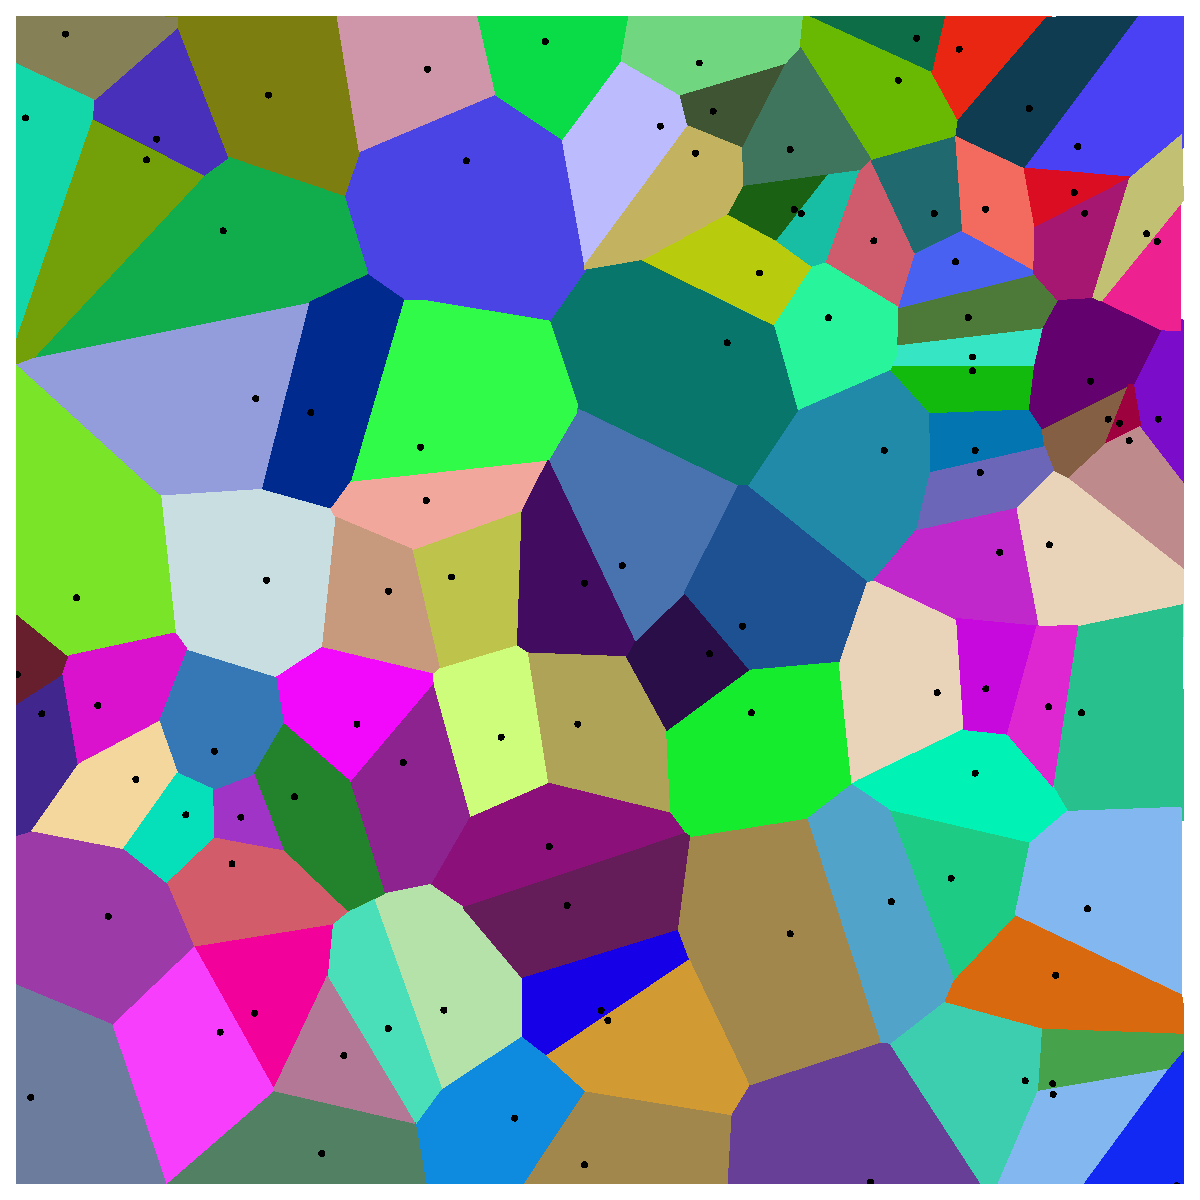
\includegraphics[width=\columnwidth]{voro2d}\\
	\centering Voronoi decomposition
	\column{0.6\textwidth}
	\centering Radial distribution function\\
	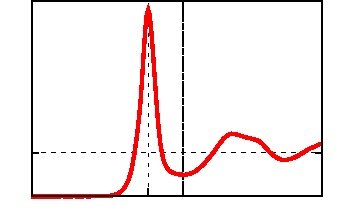
\includegraphics[width=\columnwidth]{typicalRdf}
	\begin{itemize}
		\item A bond between neighbours
		\item Voronoi is not good (anisotropy)
		\item First shell
	\end{itemize}
	\end{columns}
\end{frame}

\begin{frame}{Topology of the bond network}
	\begin{columns}
	\column{0.3\textwidth}
	\centering FCC\\
	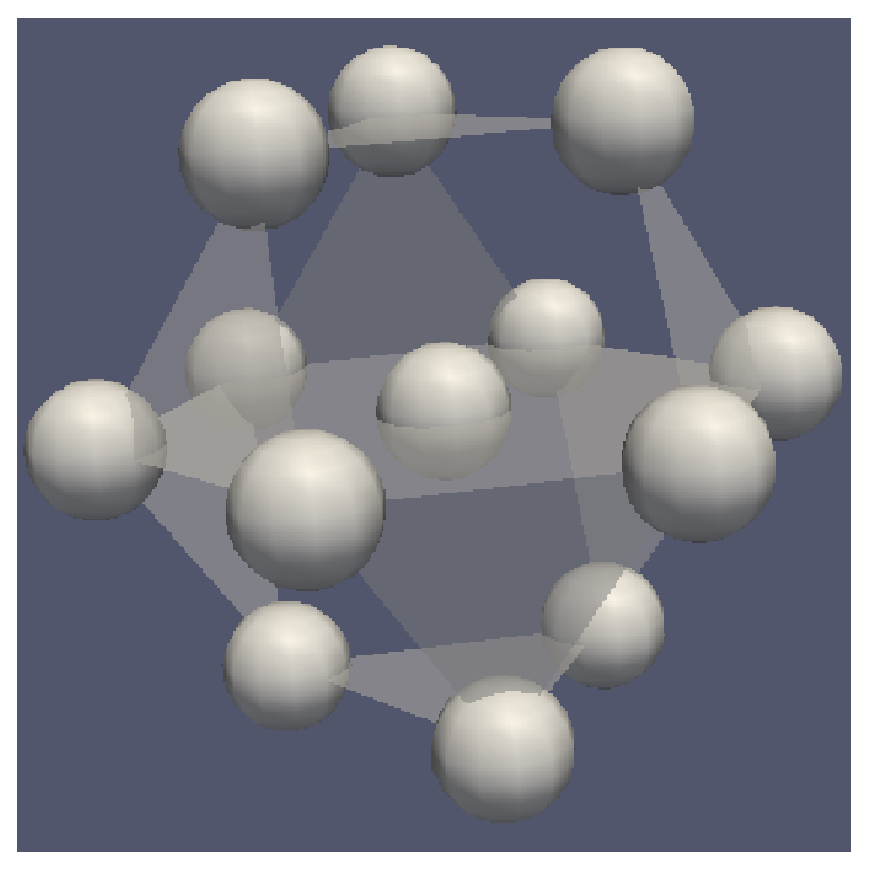
\includegraphics[width=\columnwidth]{fcc_13}
	
	\bigskip
	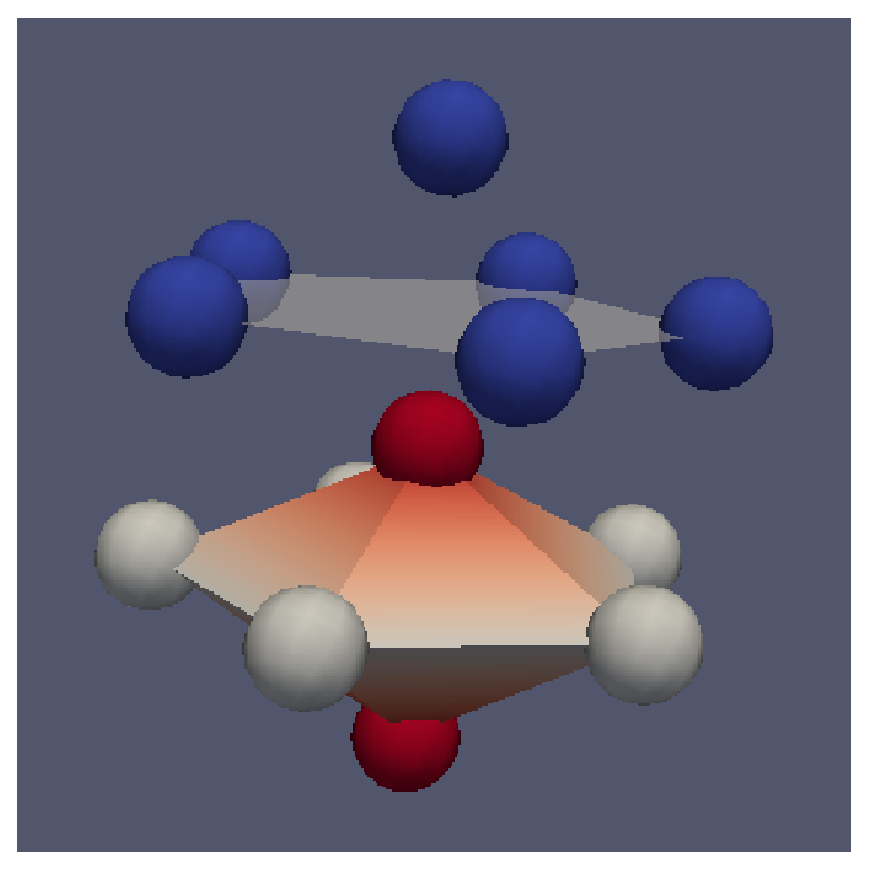
\includegraphics[width=\columnwidth]{ico_13_1551}\\
	Icosahedron
	\column{0.7\textwidth}
	\begin{itemize}
		\item Number of neighbours
		\item Voronoi signature \citep{tanemura1977geometrical}
		\item Common neighbours \citep{Honeycutt1987}
		\item Topological cluster classification \citep{Williams2007}
	\end{itemize}
	Difficult to correlate discrete categories in time or space.
	\end{columns}
\end{frame}

\subsection{Spherical harmonics}

\begin{frame}{Spherical harmonics}
	\begin{columns}
	\column{0.5\textwidth}
	\begin{itemize}
		\item Analogue to Fourier decomposition
		\item On a sphere
	\end{itemize}
	\column{0.5\textwidth}
	\[ h(\theta,\phi) = \sum_{\ell=0}^{\infty} \sum_{m=-\ell}^{\ell} q_{\ell m} Y_{\ell m}(\theta,\phi) \]
	\end{columns}
	\begin{description}
		\item[$\ell$] Order of symmetry
		\item[$m$] Orientation
		\item[$(r,\theta,\phi)$] Spherical coordinates
	\end{description}
	\begin{center}Altitude on earth: Decomposition\end{center}
	\begin{tabular}{ccc}
	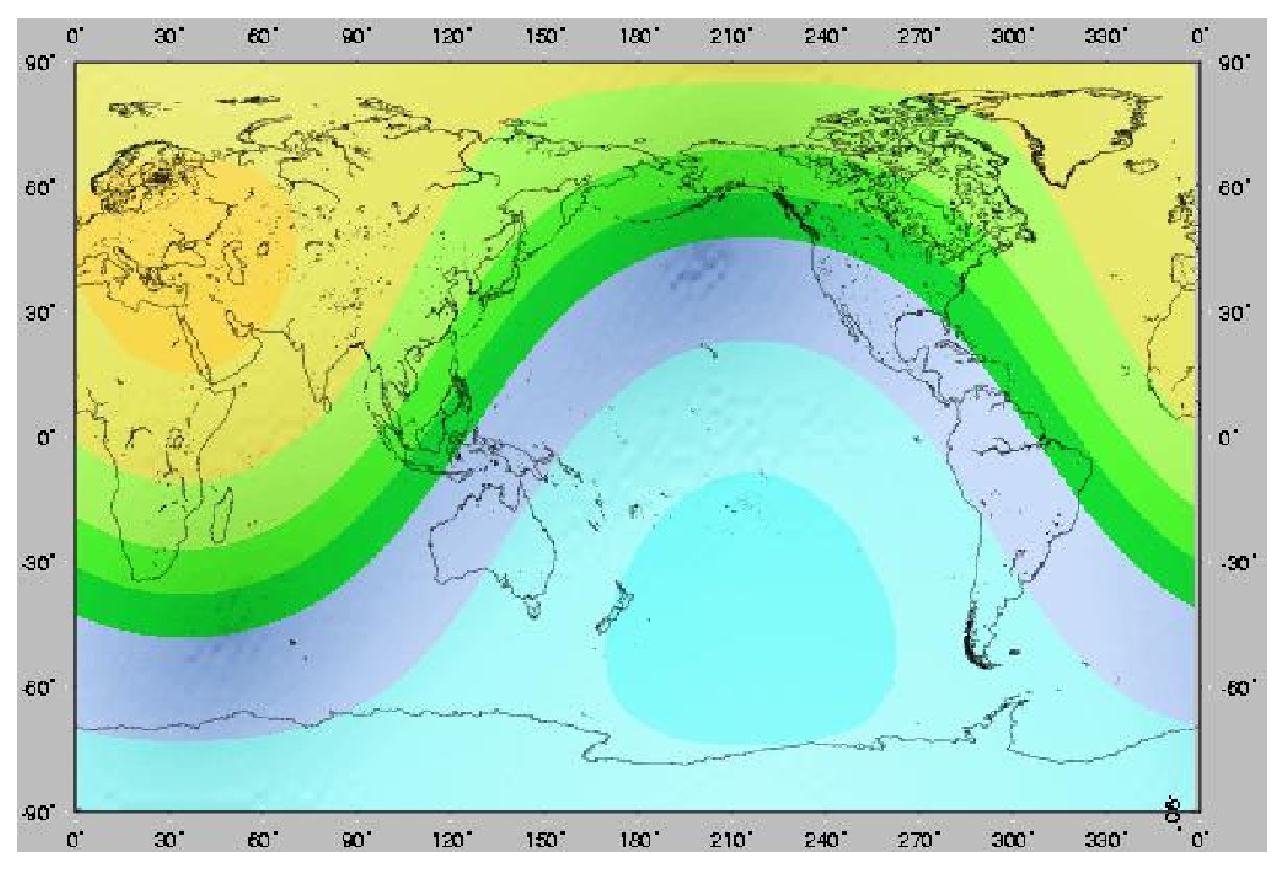
\includegraphics[width=0.3\textwidth]{earth_l1} & 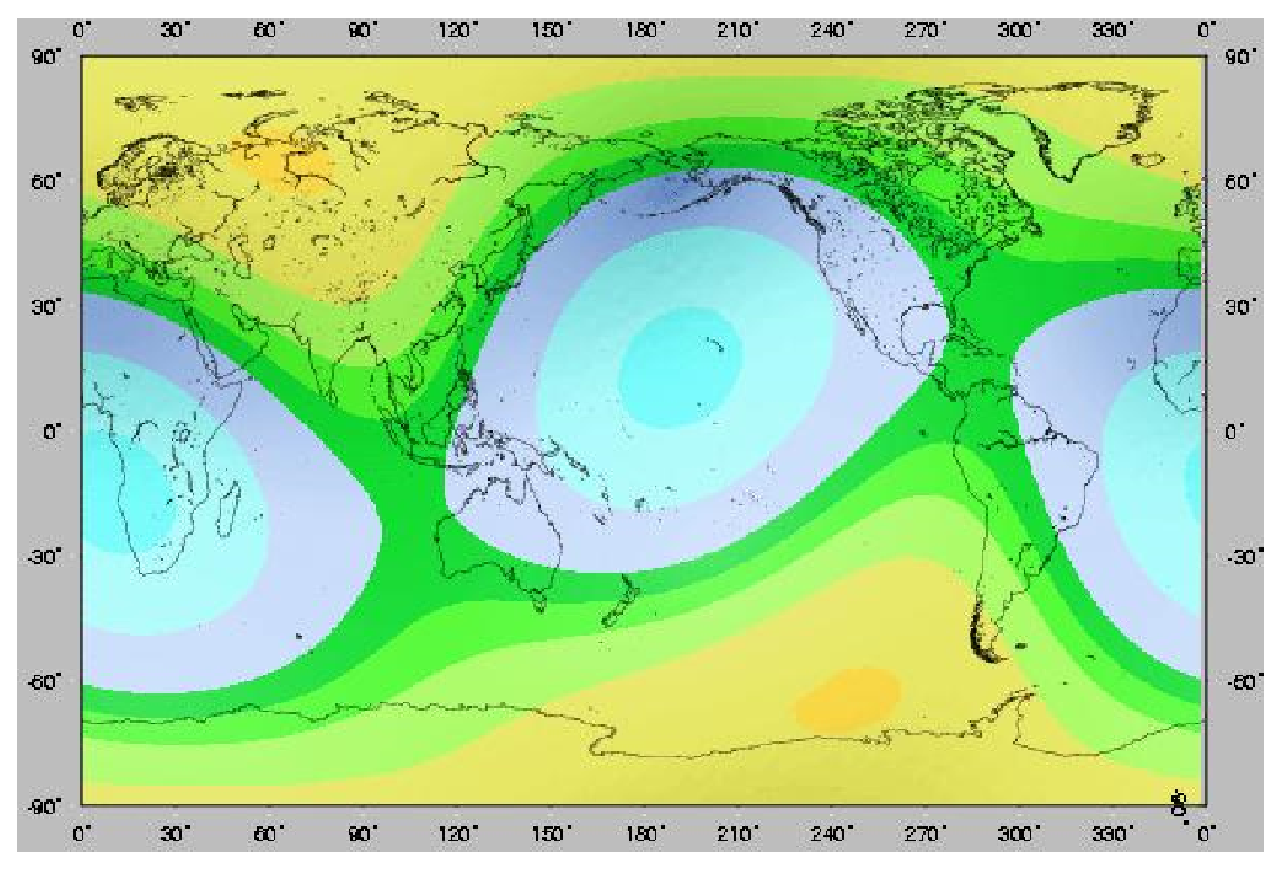
\includegraphics[width=0.3\textwidth]{earth_l2} & 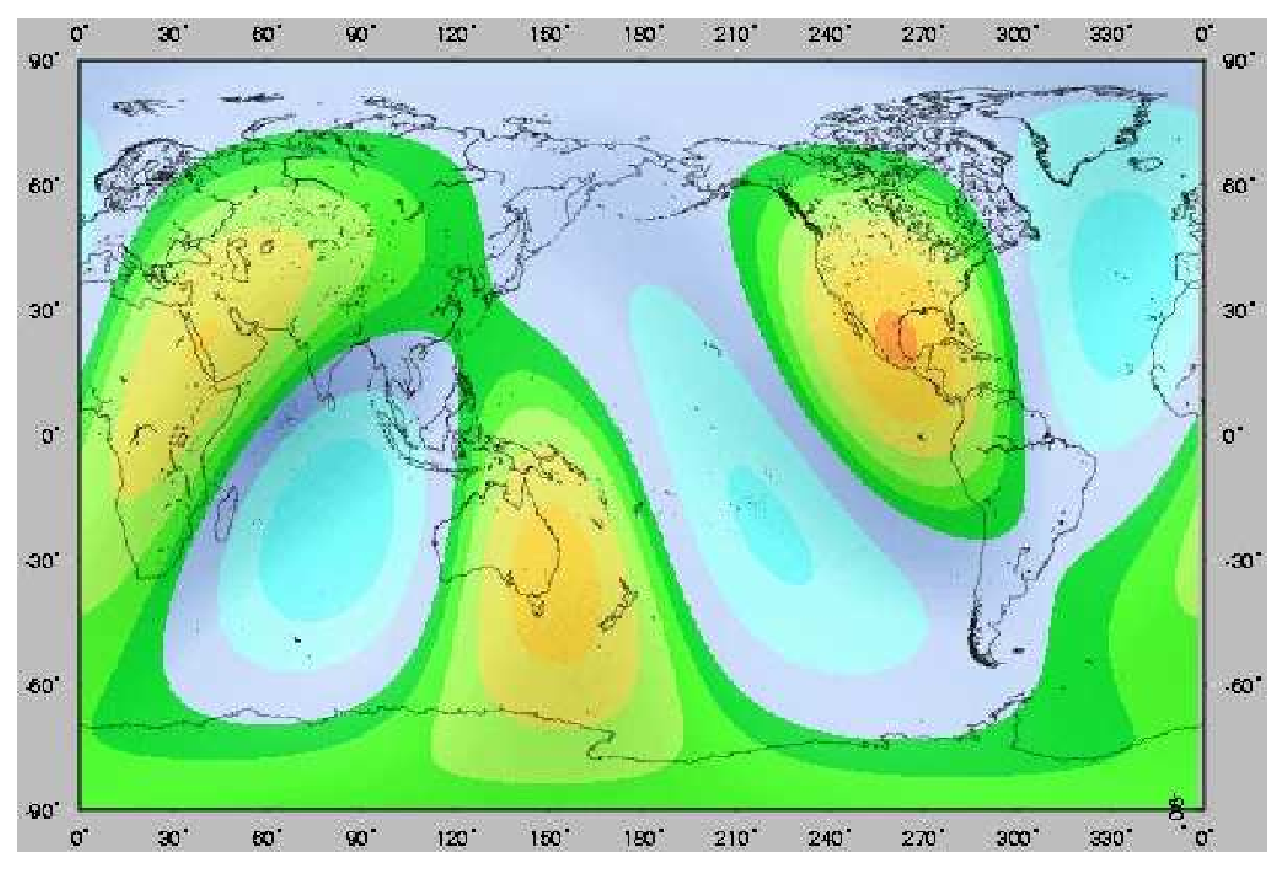
\includegraphics[width=0.3\textwidth]{earth_l3} \\ 
	$\ell=1$ & $\ell=2$ & $\ell=3$ \\ 
	\end{tabular} 
\end{frame}

\begin{frame}{Approximation by spherical harmonics}
	\begin{columns}[T]
	\centering
	\column{0.4\textwidth}
	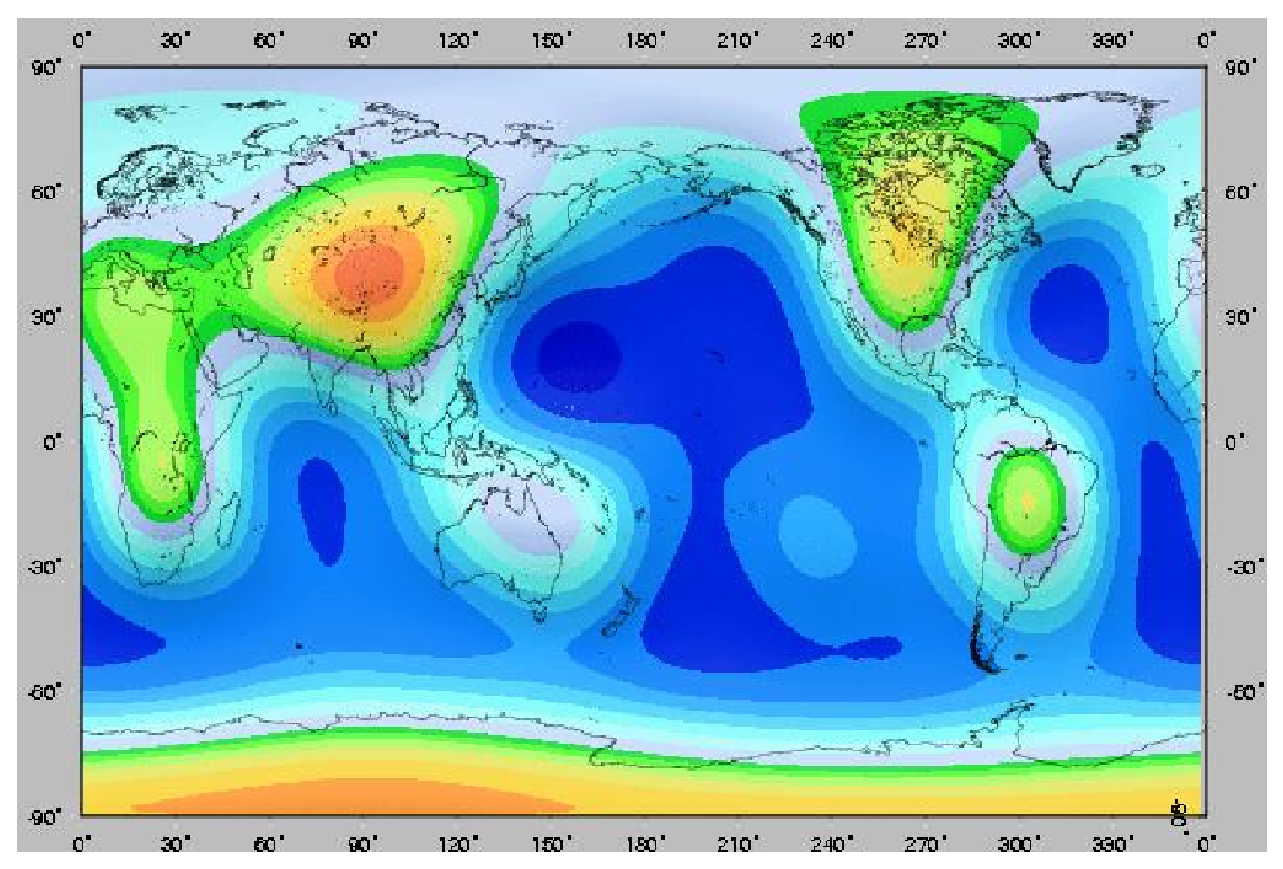
\includegraphics[width=\textwidth]{earth_to6}\\
	\centering{$\sum_{\ell=0}^6$}
	
	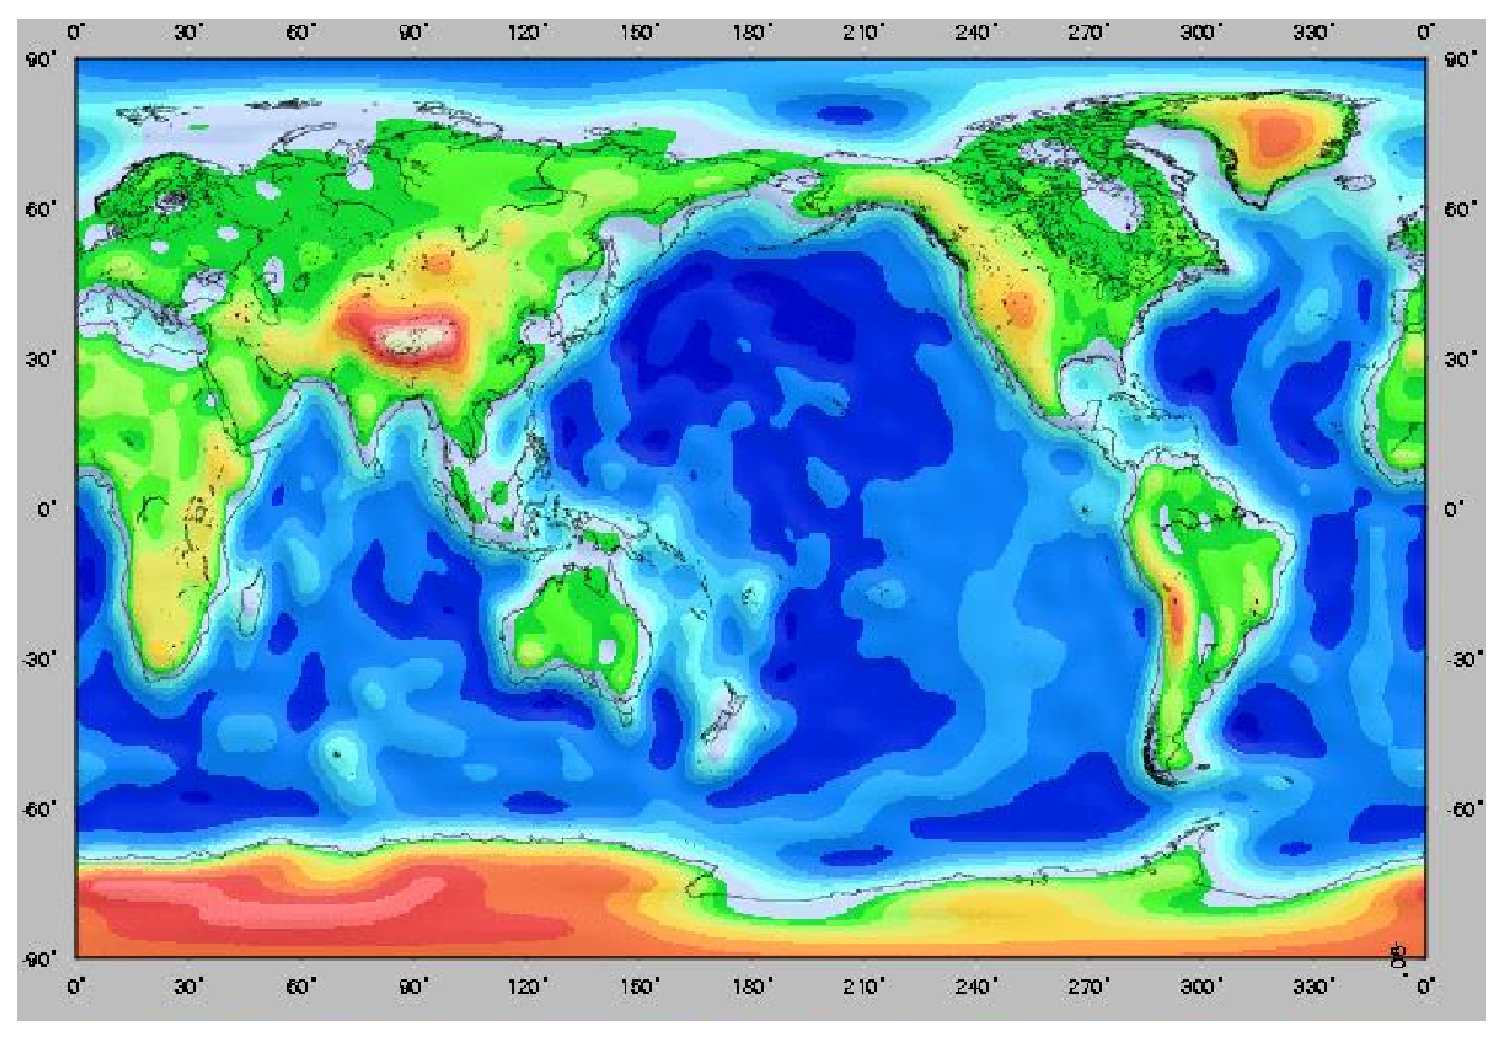
\includegraphics[width=\textwidth]{earth_to36}\\
	\centering{$\sum_{\ell=0}^{36}$}
	\column{0.4\textwidth}
	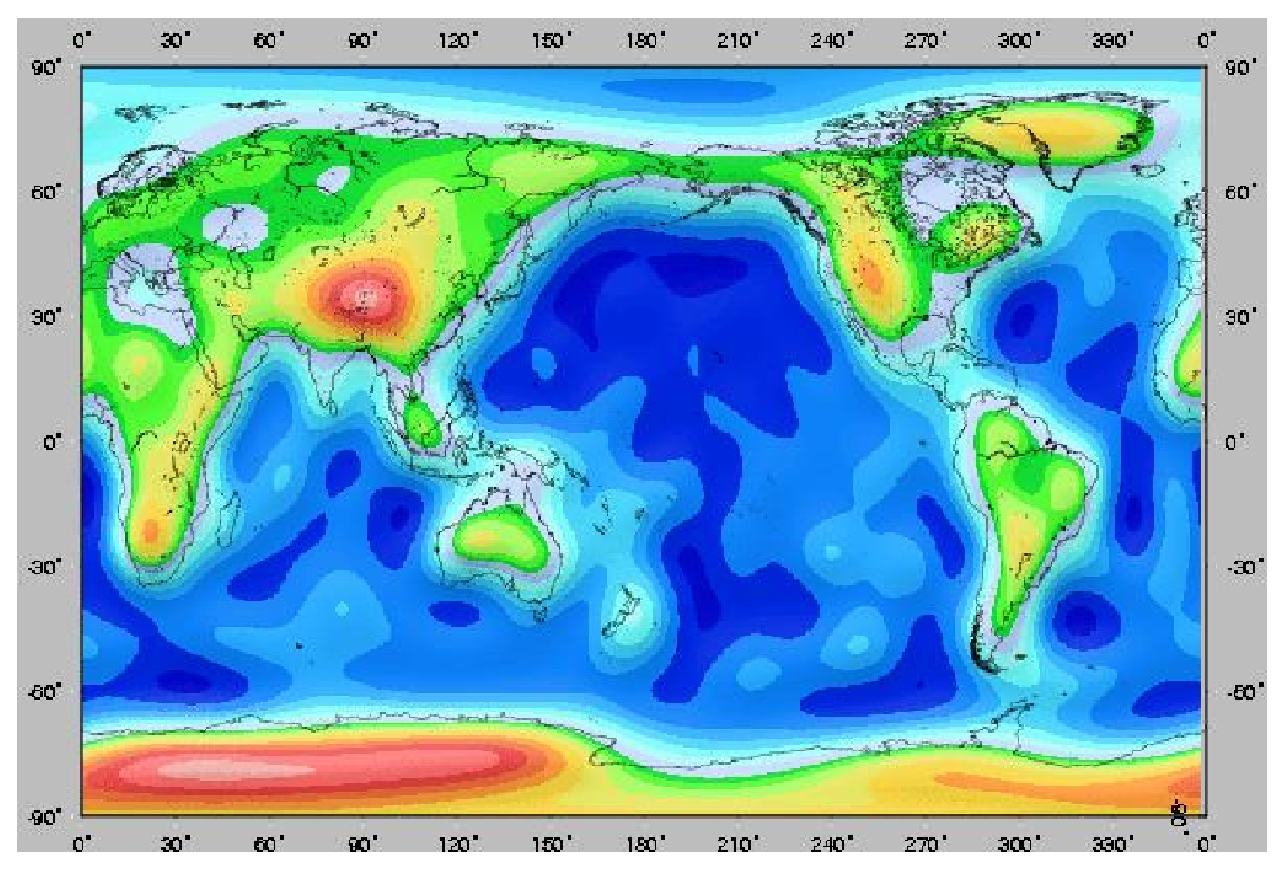
\includegraphics[width=\textwidth]{earth_to16}\\
	\centering{$\sum_{\ell=0}^{16}$}
	
	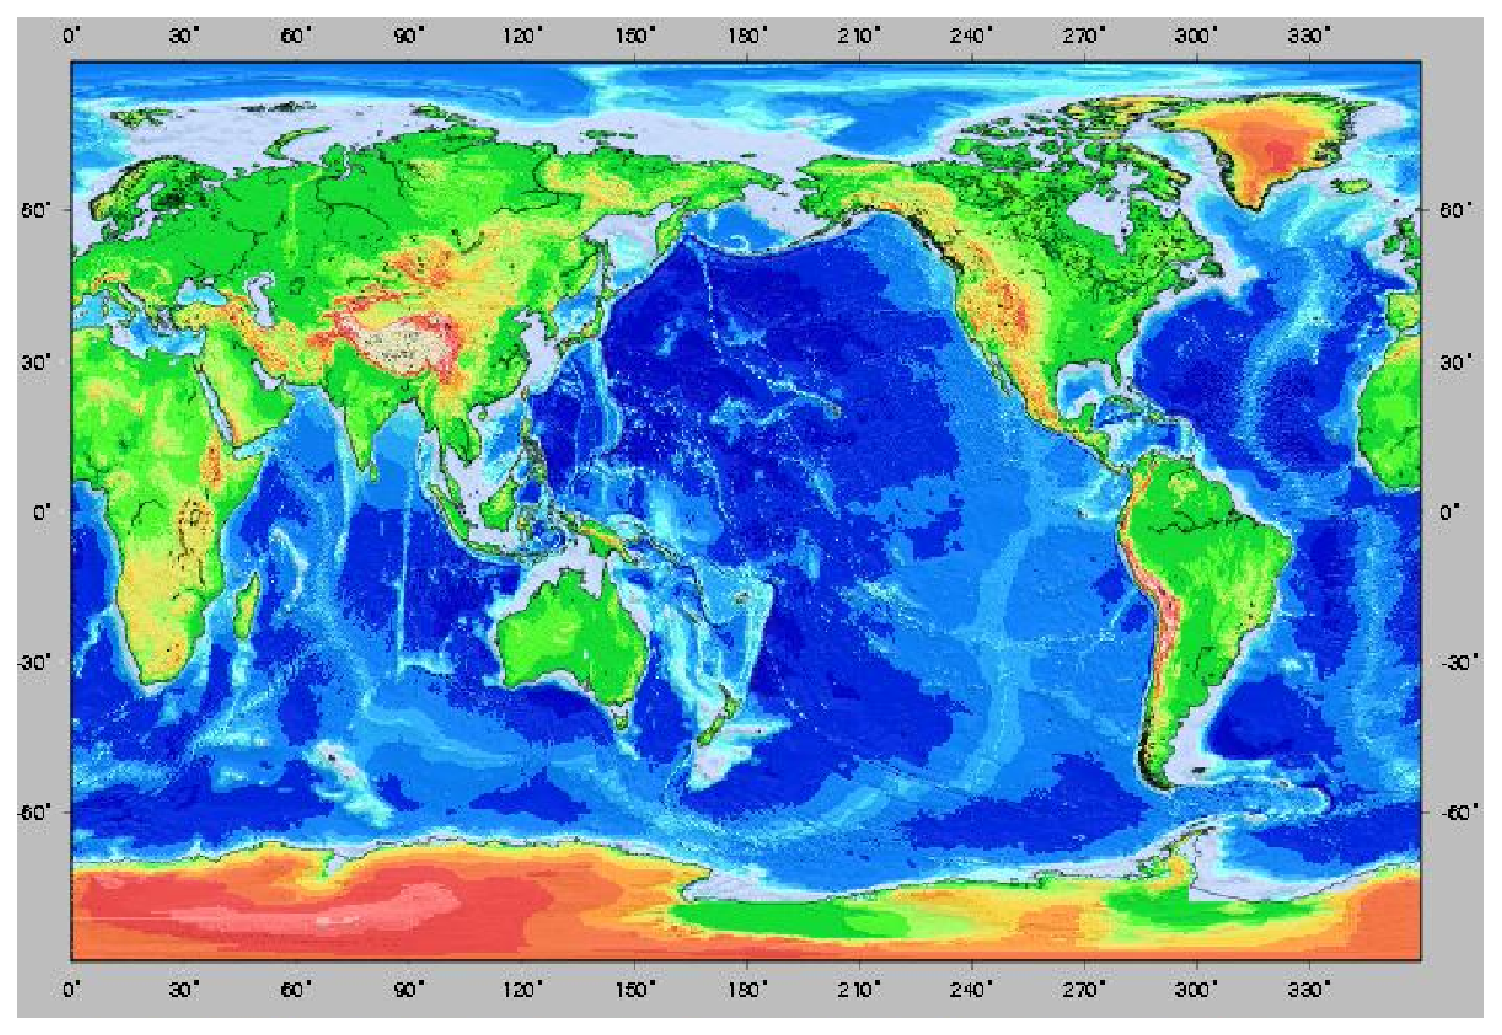
\includegraphics[width=\textwidth]{earth_grid}\\
	Full grid of earth topography
	\end{columns}
\end{frame}

\subsection{Bond orientational order}

\againframe{local_sym_sh}

\begin{frame}{Bond orientational order}
	\begin{columns}
	\column{0.5\textwidth}
	\begin{itemize}
		\item A set of spherical harmonics for each
		\begin{itemize}
			\item Bond $\vec{r}_{ij}$
			\item Neighbourhood
		\end{itemize}
		\item Rotational invariants
		\begin{itemize}
			\item Strength of the $\ell$-fold symmetry
			\item Characterise the symmetry group
		\end{itemize}
	\end{itemize}
	\column{0.5\textwidth}
	\[ q_{\ell m}(i) = \frac{1}{N_i}\sum_{j=0}^{N_i} Y_{\ell m}(\theta(\vec r_{ij}),\phi(\vec r_{ij})) \]
	\[ q_\ell = \sqrt{\frac{4\pi}{2l+1} \sum_{m=-\ell}^{\ell} |q_{\ell m}|^2 } \]
	\end{columns}
	\[w_\ell = \frac{
		\sum\limits_{m_1+m_2+m_3=0} 
			\left( \begin{array}{ccc}
				\ell & \ell & \ell \\
				m_1 & m_2 & m_3 
			\end{array} \right)
			q_{\ell m_1} q_{\ell m_2} q_{\ell m_3}
	}{
		\left(
			\sum\limits_{m=-\ell}^{\ell} |q_{\ell m}|^2
		\right)^{\frac{3}{2}}
	}\]
	
	\footnotesize{\bibentry{steinhardt1983boo}}
\end{frame}

\begin{frame}{Invariants distributions}
	\begin{columns}
	\column{0.6\textwidth}
	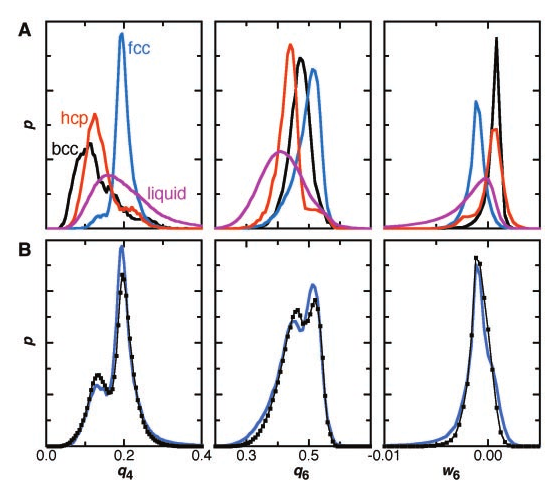
\includegraphics[width=\columnwidth]{gasser_invariants}
	\column{0.4\textwidth}
	\begin{itemize}
		\item Distributions are
		\begin{itemize}
			\item Noisy
			\item Broad
			\item Overlapping
		\end{itemize}
		\item Can characterize a sample
		\item Cannot characterize a single particle
	\end{itemize}
	\end{columns}
	\footnotesize{\bibentry{Gasser2001}}
\end{frame}

\begin{frame}{Coarse-grained BOO}
	\begin{columns}
	\column{0.6\textwidth}
	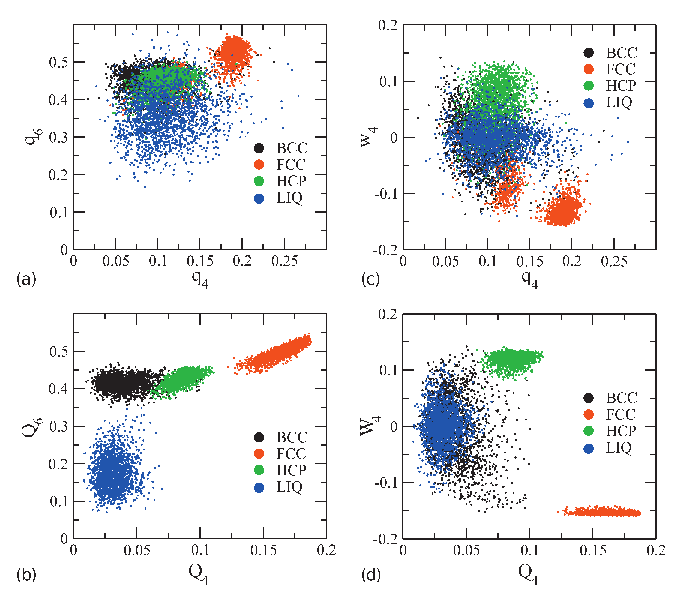
\includegraphics[width=\columnwidth]{invariants_maps_raster}
	\column{0.4\textwidth}
	\[ Q_{\ell m}(i) = \frac{1}{\tilde{N} (i)} \sum_{k=0}^{\tilde{N}(i)} q_{\ell m}(k) \]
	\begin{itemize}
		\item Take into account the second shell
		\item Structures with some periodicity are much better defined
		\item Non periodic structures goes to zeros
	\end{itemize}
	\end{columns}
	\footnotesize{\bibentry{lechner:114707}}
\end{frame}

\subsection{Lifetime}

\begin{frame}{Time correlation}
	\begin{itemize}
	\item Time auto-correlation of the bond order
	\[
	g_\ell(t) \equiv \left\langle \frac{
		\sum_{m=-\ell}^{\ell} q_{\ell m}(i, t_0) q_{\ell m}^{*}(i, t_0+t)
	}{
		\sqrt{\sum_{m=-\ell}^{\ell} \left\|q_{\ell m}(i,t_0)\right\|^2}
	}\right\rangle_{i, t_0}
	\]
	\item Can be done with the $Q_{\ell m}$ to discard aperiodic structures $\Longrightarrow G_\ell(t)$
	\item The ratio $G_\ell(t)/g_\ell(t)<1$ gives the proportion of $t$-lived structures that are periodic
	\end{itemize}
\end{frame}

\begin{frame}{Lifetimes}
	\begin{textblock*}{0.6\textwidth}(10mm,92mm)
		\simplephasediagram{}
	\end{textblock*}
	%\tikz[baseline, remember picture]\node[anchor=base] (text)%
	%		{Near $\phi_g$ and $\tau_\alpha$, MRCO live longer than icosahedra};
	\tikzstyle{background grid}=[draw, black!50,step=0.1\textwidth]
	\begin{center}
    \begin{tikzpicture}%, show background grid]
		\node [inner sep=0pt,above right] 
			{\resizebox{0.7\textwidth}{!}{% GNUPLOT: LaTeX picture with Postscript
\begingroup
  \makeatletter
  \providecommand\color[2][]{%
    \GenericError{(gnuplot) \space\space\space\@spaces}{%
      Package color not loaded in conjunction with
      terminal option `colourtext'%
    }{See the gnuplot documentation for explanation.%
    }{Either use 'blacktext' in gnuplot or load the package
      color.sty in LaTeX.}%
    \renewcommand\color[2][]{}%
  }%
  \providecommand\includegraphics[2][]{%
    \GenericError{(gnuplot) \space\space\space\@spaces}{%
      Package graphicx or graphics not loaded%
    }{See the gnuplot documentation for explanation.%
    }{The gnuplot epslatex terminal needs graphicx.sty or graphics.sty.}%
    \renewcommand\includegraphics[2][]{}%
  }%
  \providecommand\rotatebox[2]{#2}%
  \@ifundefined{ifGPcolor}{%
    \newif\ifGPcolor
    \GPcolortrue
  }{}%
  \@ifundefined{ifGPblacktext}{%
    \newif\ifGPblacktext
    \GPblacktexttrue
  }{}%
  % define a \g@addto@macro without @ in the name:
  \let\gplgaddtomacro\g@addto@macro
  % define empty templates for all commands taking text:
  \gdef\gplbacktext{}%
  \gdef\gplfronttext{}%
  \makeatother
  \ifGPblacktext
    % no textcolor at all
    \def\colorrgb#1{}%
    \def\colorgray#1{}%
  \else
    % gray or color?
    \ifGPcolor
      \def\colorrgb#1{\color[rgb]{#1}}%
      \def\colorgray#1{\color[gray]{#1}}%
      \expandafter\def\csname LTw\endcsname{\color{white}}%
      \expandafter\def\csname LTb\endcsname{\color{black}}%
      \expandafter\def\csname LTa\endcsname{\color{black}}%
      \expandafter\def\csname LT0\endcsname{\color[rgb]{1,0,0}}%
      \expandafter\def\csname LT1\endcsname{\color[rgb]{0,1,0}}%
      \expandafter\def\csname LT2\endcsname{\color[rgb]{0,0,1}}%
      \expandafter\def\csname LT3\endcsname{\color[rgb]{1,0,1}}%
      \expandafter\def\csname LT4\endcsname{\color[rgb]{0,1,1}}%
      \expandafter\def\csname LT5\endcsname{\color[rgb]{1,1,0}}%
      \expandafter\def\csname LT6\endcsname{\color[rgb]{0,0,0}}%
      \expandafter\def\csname LT7\endcsname{\color[rgb]{1,0.3,0}}%
      \expandafter\def\csname LT8\endcsname{\color[rgb]{0.5,0.5,0.5}}%
    \else
      % gray
      \def\colorrgb#1{\color{black}}%
      \def\colorgray#1{\color[gray]{#1}}%
      \expandafter\def\csname LTw\endcsname{\color{white}}%
      \expandafter\def\csname LTb\endcsname{\color{black}}%
      \expandafter\def\csname LTa\endcsname{\color{black}}%
      \expandafter\def\csname LT0\endcsname{\color{black}}%
      \expandafter\def\csname LT1\endcsname{\color{black}}%
      \expandafter\def\csname LT2\endcsname{\color{black}}%
      \expandafter\def\csname LT3\endcsname{\color{black}}%
      \expandafter\def\csname LT4\endcsname{\color{black}}%
      \expandafter\def\csname LT5\endcsname{\color{black}}%
      \expandafter\def\csname LT6\endcsname{\color{black}}%
      \expandafter\def\csname LT7\endcsname{\color{black}}%
      \expandafter\def\csname LT8\endcsname{\color{black}}%
    \fi
  \fi
  \setlength{\unitlength}{0.0500bp}%
  \begin{picture}(7200.00,5040.00)%
    \gplgaddtomacro\gplbacktext{%
      \csname LTb\endcsname%
      \put(1122,3995){\makebox(0,0)[r]{\strut{}$0.4$}}%
      \put(1122,4255){\makebox(0,0)[r]{\strut{}$0.5$}}%
      \put(1122,4516){\makebox(0,0)[r]{\strut{}$0.6$}}%
      \put(1122,4776){\makebox(0,0)[r]{\strut{}$0.7$}}%
      \put(440,4278){\rotatebox{-270}{\makebox(0,0){\strut{}}}}%
      \put(6979,4278){\rotatebox{-270}{\makebox(0,0){\strut{}}}}%
      \put(4007,3714){\makebox(0,0){\strut{}}}%
      \put(4007,4666){\makebox(0,0){\strut{}}}%
      \put(4007,4665){\makebox(0,0){\strut{}}}%
      \put(330,3890){\makebox(0,0)[l]{\strut{}}}%
      \put(4007,4278){\makebox(0,0){\strut{}$\ell=4$}}%
    }%
    \gplgaddtomacro\gplfronttext{%
    }%
    \gplgaddtomacro\gplbacktext{%
      \csname LTb\endcsname%
      \put(1122,2689){\makebox(0,0)[r]{\strut{}$0.5$}}%
      \put(1122,3234){\makebox(0,0)[r]{\strut{}$0.6$}}%
      \put(1122,3779){\makebox(0,0)[r]{\strut{}$0.7$}}%
      \put(440,3149){\rotatebox{-270}{\makebox(0,0){\strut{}}}}%
      \put(6979,3149){\rotatebox{-270}{\makebox(0,0){\strut{}}}}%
      \put(4007,2454){\makebox(0,0){\strut{}}}%
      \put(4007,3669){\makebox(0,0){\strut{}}}%
      \put(4007,3668){\makebox(0,0){\strut{}}}%
      \put(330,2630){\makebox(0,0)[l]{\strut{}}}%
      \put(4007,3150){\makebox(0,0){\strut{}$\ell=6$}}%
    }%
    \gplgaddtomacro\gplfronttext{%
      \csname LTb\endcsname%
      \put(5773,2693){\makebox(0,0)[r]{\strut{}$\phi=0.497$}}%
      \csname LTb\endcsname%
      \put(5773,2913){\makebox(0,0)[r]{\strut{}$\phi=0.535$}}%
      \csname LTb\endcsname%
      \put(5773,3133){\makebox(0,0)[r]{\strut{}$\phi=0.555$}}%
      \csname LTb\endcsname%
      \put(5773,3353){\makebox(0,0)[r]{\strut{}$\phi=0.576$}}%
    }%
    \gplgaddtomacro\gplbacktext{%
      \csname LTb\endcsname%
      \put(1122,1460){\makebox(0,0)[r]{\strut{}$0.6$}}%
      \put(1122,1813){\makebox(0,0)[r]{\strut{}$0.7$}}%
      \put(1122,2166){\makebox(0,0)[r]{\strut{}$0.8$}}%
      \put(1122,2519){\makebox(0,0)[r]{\strut{}$0.9$}}%
      \put(440,1889){\rotatebox{-270}{\makebox(0,0){\strut{}}}}%
      \put(6979,1889){\rotatebox{-270}{\makebox(0,0){\strut{}}}}%
      \put(4007,1194){\makebox(0,0){\strut{}}}%
      \put(4007,2409){\makebox(0,0){\strut{}}}%
      \put(4007,2408){\makebox(0,0){\strut{}}}%
      \put(330,1370){\makebox(0,0)[l]{\strut{}}}%
      \put(4007,1890){\makebox(0,0){\strut{}$\ell=8$}}%
      \put(1529,2267){\makebox(0,0)[l]{\strut{}$\frac{G_\ell(t)}{g_\ell(t)}$}}%
    }%
    \gplgaddtomacro\gplfronttext{%
    }%
    \gplgaddtomacro\gplbacktext{%
      \csname LTb\endcsname%
      \put(1122,534){\makebox(0,0)[r]{\strut{}$0.3$}}%
      \put(1122,775){\makebox(0,0)[r]{\strut{}$0.4$}}%
      \put(1122,1017){\makebox(0,0)[r]{\strut{}$0.5$}}%
      \put(1122,1259){\makebox(0,0)[r]{\strut{}$0.6$}}%
      \put(1316,220){\makebox(0,0){\strut{}$10^{0}$}}%
      \put(2677,220){\makebox(0,0){\strut{}$10^{1}$}}%
      \put(4038,220){\makebox(0,0){\strut{}$10^{2}$}}%
      \put(5399,220){\makebox(0,0){\strut{}$10^{3}$}}%
      \put(6760,220){\makebox(0,0){\strut{}$10^{4}$}}%
      \put(440,849){\rotatebox{-270}{\makebox(0,0){\strut{}}}}%
      \put(6979,849){\rotatebox{-270}{\makebox(0,0){\strut{}}}}%
      \put(4007,-66){\makebox(0,0){\strut{}}}%
      \put(4007,1149){\makebox(0,0){\strut{}}}%
      \put(4007,1148){\makebox(0,0){\strut{}}}%
      \put(330,110){\makebox(0,0)[l]{\strut{}}}%
      \put(4007,850){\makebox(0,0){\strut{}$\ell=10$}}%
    }%
    \gplgaddtomacro\gplfronttext{%
    }%
    \gplbacktext
    \put(0,0){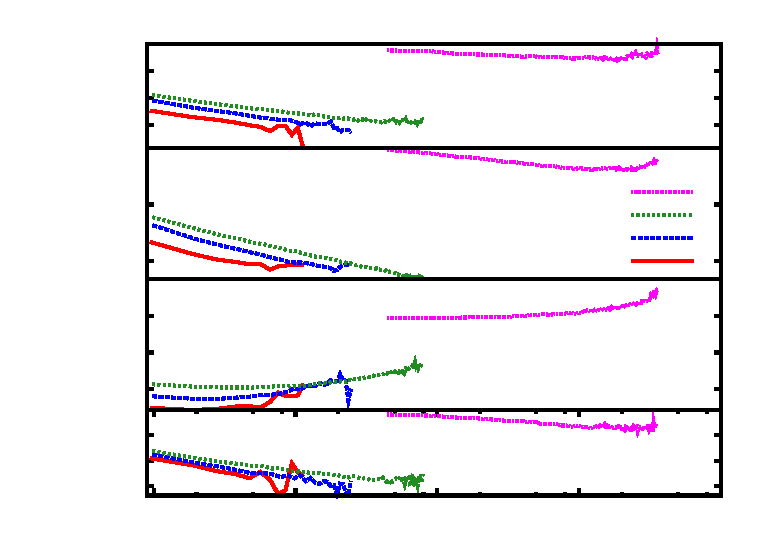
\includegraphics{Qlm_qlm_correl_ratio}}%
    \gplfronttext
  \end{picture}%
\endgroup
}};
		%\node [rectangle, red, minimum width=0.08\textwidth, minimum height=0.05\textwidth, draw] at (0.3\textwidth, 0.4\textwidth) (q4) {};
		\node [rectangle, red, minimum width=0.08\textwidth, minimum height=0.05\textwidth, draw] at (0.6\textwidth, 0.4\textwidth) (q6) {};
		\node at (0.35\textwidth, 0.525\textwidth) (text)%
			{Near $\phi_g$ and $\tau_\alpha$, MRCO live longer than icosahedra};
		%\path[->] (text) edge (q4);
		\path[->] (text.east) edge [out=-45, in=0] (q6.east);
	\end{tikzpicture}
	\begin{description}
		\item[$\ell=8\nearrow$] No long-lived aperiodic $8$-fold
		\item[$\ell=10\searrow$] No long lived periodic $10$-fold
	\end{description}
	\end{center}
\end{frame}

\subsection{Spatial correlation}

\begin{frame}{Spatial correlation}
	\begin{itemize}
		\item Correlation of the bond order between particles $i$ and $j$
		\[ s_\ell(i,j) = \frac{
			\sum_{m=-\ell}^{\ell} q_{\ell m}(i) q_{\ell m}^{*}(j)
		}{
			\sqrt{\sum_{m=-\ell}^{\ell} |q_{\ell m}(i)|^2} \sqrt{\sum_{m=-\ell}^{\ell} |q_{\ell m}(j)|^2}
		}\]
		\item Spatial correlation
		\[ g_\ell(r) \equiv \frac{1}{N}\sum_i^N \frac{
			\sum_{j \neq i}{ s_\ell(i,j) \delta\left(\left\|\vec{r}_i-\vec{r}_j \right\| - r \right)}
		}{
		\sum_{j \neq i}{\delta\left(\left\|\vec{r}_i-\vec{r}_j \right\| - r \right)}
		} \]
		\item Can be done with the $Q_{\ell m}$ to discard aperiodic structures $\Longrightarrow G_\ell(r)$
	\end{itemize}
\end{frame}

\begin{frame}{Size of the crystal-like ordered regions}
	\begin{textblock*}{0.6\textwidth}(10mm,92mm)
		\simplephasediagram{}
	\end{textblock*}
	\begin{columns}
	\column{0.5\textwidth}
	\resizebox{\columnwidth}{!}{\begin{LARGE}% GNUPLOT: LaTeX picture with Postscript
\begingroup
  \makeatletter
  \providecommand\color[2][]{%
    \GenericError{(gnuplot) \space\space\space\@spaces}{%
      Package color not loaded in conjunction with
      terminal option `colourtext'%
    }{See the gnuplot documentation for explanation.%
    }{Either use 'blacktext' in gnuplot or load the package
      color.sty in LaTeX.}%
    \renewcommand\color[2][]{}%
  }%
  \providecommand\includegraphics[2][]{%
    \GenericError{(gnuplot) \space\space\space\@spaces}{%
      Package graphicx or graphics not loaded%
    }{See the gnuplot documentation for explanation.%
    }{The gnuplot epslatex terminal needs graphicx.sty or graphics.sty.}%
    \renewcommand\includegraphics[2][]{}%
  }%
  \providecommand\rotatebox[2]{#2}%
  \@ifundefined{ifGPcolor}{%
    \newif\ifGPcolor
    \GPcolortrue
  }{}%
  \@ifundefined{ifGPblacktext}{%
    \newif\ifGPblacktext
    \GPblacktexttrue
  }{}%
  % define a \g@addto@macro without @ in the name:
  \let\gplgaddtomacro\g@addto@macro
  % define empty templates for all commands taking text:
  \gdef\gplbacktext{}%
  \gdef\gplfronttext{}%
  \makeatother
  \ifGPblacktext
    % no textcolor at all
    \def\colorrgb#1{}%
    \def\colorgray#1{}%
  \else
    % gray or color?
    \ifGPcolor
      \def\colorrgb#1{\color[rgb]{#1}}%
      \def\colorgray#1{\color[gray]{#1}}%
      \expandafter\def\csname LTw\endcsname{\color{white}}%
      \expandafter\def\csname LTb\endcsname{\color{black}}%
      \expandafter\def\csname LTa\endcsname{\color{black}}%
      \expandafter\def\csname LT0\endcsname{\color[rgb]{1,0,0}}%
      \expandafter\def\csname LT1\endcsname{\color[rgb]{0,1,0}}%
      \expandafter\def\csname LT2\endcsname{\color[rgb]{0,0,1}}%
      \expandafter\def\csname LT3\endcsname{\color[rgb]{1,0,1}}%
      \expandafter\def\csname LT4\endcsname{\color[rgb]{0,1,1}}%
      \expandafter\def\csname LT5\endcsname{\color[rgb]{1,1,0}}%
      \expandafter\def\csname LT6\endcsname{\color[rgb]{0,0,0}}%
      \expandafter\def\csname LT7\endcsname{\color[rgb]{1,0.3,0}}%
      \expandafter\def\csname LT8\endcsname{\color[rgb]{0.5,0.5,0.5}}%
    \else
      % gray
      \def\colorrgb#1{\color{black}}%
      \def\colorgray#1{\color[gray]{#1}}%
      \expandafter\def\csname LTw\endcsname{\color{white}}%
      \expandafter\def\csname LTb\endcsname{\color{black}}%
      \expandafter\def\csname LTa\endcsname{\color{black}}%
      \expandafter\def\csname LT0\endcsname{\color{black}}%
      \expandafter\def\csname LT1\endcsname{\color{black}}%
      \expandafter\def\csname LT2\endcsname{\color{black}}%
      \expandafter\def\csname LT3\endcsname{\color{black}}%
      \expandafter\def\csname LT4\endcsname{\color{black}}%
      \expandafter\def\csname LT5\endcsname{\color{black}}%
      \expandafter\def\csname LT6\endcsname{\color{black}}%
      \expandafter\def\csname LT7\endcsname{\color{black}}%
      \expandafter\def\csname LT8\endcsname{\color{black}}%
    \fi
  \fi
  \setlength{\unitlength}{0.0500bp}%
  \begin{picture}(7200.00,5040.00)%
    \gplgaddtomacro\gplbacktext{%
      \csname LTb\endcsname%
      \put(1056,704){\makebox(0,0)[r]{\strut{}$10^{-7}$}}%
      \put(1056,1518){\makebox(0,0)[r]{\strut{}$10^{-6}$}}%
      \put(1056,2333){\makebox(0,0)[r]{\strut{}$10^{-5}$}}%
      \put(1056,3147){\makebox(0,0)[r]{\strut{}$10^{-4}$}}%
      \put(1056,3962){\makebox(0,0)[r]{\strut{}$10^{-3}$}}%
      \put(1056,4776){\makebox(0,0)[r]{\strut{}$10^{-2}$}}%
      \put(1453,484){\makebox(0,0){\strut{}$2$}}%
      \put(2117,484){\makebox(0,0){\strut{}$2.5$}}%
      \put(2780,484){\makebox(0,0){\strut{}$3$}}%
      \put(3443,484){\makebox(0,0){\strut{}$3.5$}}%
      \put(4107,484){\makebox(0,0){\strut{}$4$}}%
      \put(4770,484){\makebox(0,0){\strut{}$4.5$}}%
      \put(5433,484){\makebox(0,0){\strut{}$5$}}%
      \put(6097,484){\makebox(0,0){\strut{}$5.5$}}%
      \put(6760,484){\makebox(0,0){\strut{}$6$}}%
      \put(286,2740){\rotatebox{-270}{\makebox(0,0){\strut{}$G_6(r)$}}}%
      \put(6979,2740){\rotatebox{-270}{\makebox(0,0){\strut{}}}}%
      \put(3974,154){\makebox(0,0){\strut{}$r/\sigma$}}%
      \put(3974,4666){\makebox(0,0){\strut{}}}%
      \put(3974,4665){\makebox(0,0){\strut{}}}%
      \put(-264,110){\makebox(0,0)[l]{\strut{}}}%
    }%
    \gplgaddtomacro\gplfronttext{%
      \csname LTb\endcsname%
      \put(2904,932){\makebox(0,0)[r]{\strut{}$\phi=0.535$}}%
      \csname LTb\endcsname%
      \put(2904,1262){\makebox(0,0)[r]{\strut{}$\phi=0.555$}}%
      \csname LTb\endcsname%
      \put(2904,1592){\makebox(0,0)[r]{\strut{}$\phi=0.576$}}%
    }%
    \gplbacktext
    \put(0,0){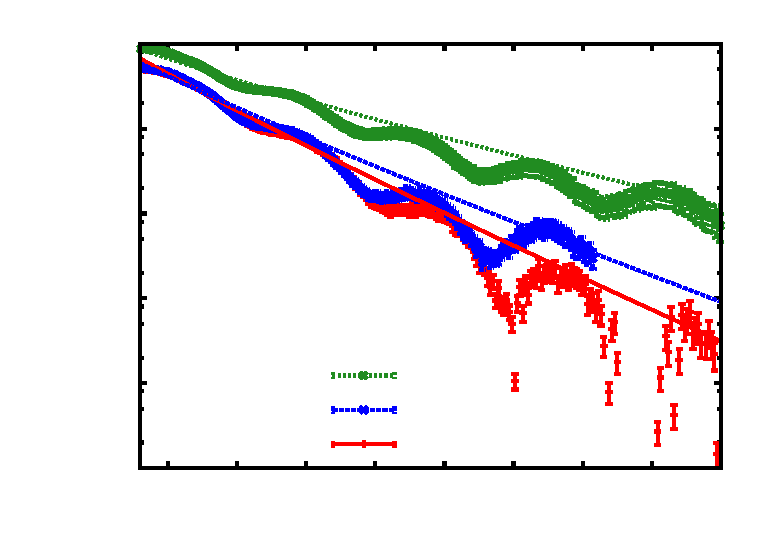
\includegraphics{fit_G6}}%
    \gplfronttext
  \end{picture}%
\endgroup
\end{LARGE}}\\
	\resizebox{\columnwidth}{!}{\begin{LARGE}% GNUPLOT: LaTeX picture with Postscript
\begingroup
  \makeatletter
  \providecommand\color[2][]{%
    \GenericError{(gnuplot) \space\space\space\@spaces}{%
      Package color not loaded in conjunction with
      terminal option `colourtext'%
    }{See the gnuplot documentation for explanation.%
    }{Either use 'blacktext' in gnuplot or load the package
      color.sty in LaTeX.}%
    \renewcommand\color[2][]{}%
  }%
  \providecommand\includegraphics[2][]{%
    \GenericError{(gnuplot) \space\space\space\@spaces}{%
      Package graphicx or graphics not loaded%
    }{See the gnuplot documentation for explanation.%
    }{The gnuplot epslatex terminal needs graphicx.sty or graphics.sty.}%
    \renewcommand\includegraphics[2][]{}%
  }%
  \providecommand\rotatebox[2]{#2}%
  \@ifundefined{ifGPcolor}{%
    \newif\ifGPcolor
    \GPcolortrue
  }{}%
  \@ifundefined{ifGPblacktext}{%
    \newif\ifGPblacktext
    \GPblacktexttrue
  }{}%
  % define a \g@addto@macro without @ in the name:
  \let\gplgaddtomacro\g@addto@macro
  % define empty templates for all commands taking text:
  \gdef\gplbacktext{}%
  \gdef\gplfronttext{}%
  \makeatother
  \ifGPblacktext
    % no textcolor at all
    \def\colorrgb#1{}%
    \def\colorgray#1{}%
  \else
    % gray or color?
    \ifGPcolor
      \def\colorrgb#1{\color[rgb]{#1}}%
      \def\colorgray#1{\color[gray]{#1}}%
      \expandafter\def\csname LTw\endcsname{\color{white}}%
      \expandafter\def\csname LTb\endcsname{\color{black}}%
      \expandafter\def\csname LTa\endcsname{\color{black}}%
      \expandafter\def\csname LT0\endcsname{\color[rgb]{1,0,0}}%
      \expandafter\def\csname LT1\endcsname{\color[rgb]{0,1,0}}%
      \expandafter\def\csname LT2\endcsname{\color[rgb]{0,0,1}}%
      \expandafter\def\csname LT3\endcsname{\color[rgb]{1,0,1}}%
      \expandafter\def\csname LT4\endcsname{\color[rgb]{0,1,1}}%
      \expandafter\def\csname LT5\endcsname{\color[rgb]{1,1,0}}%
      \expandafter\def\csname LT6\endcsname{\color[rgb]{0,0,0}}%
      \expandafter\def\csname LT7\endcsname{\color[rgb]{1,0.3,0}}%
      \expandafter\def\csname LT8\endcsname{\color[rgb]{0.5,0.5,0.5}}%
    \else
      % gray
      \def\colorrgb#1{\color{black}}%
      \def\colorgray#1{\color[gray]{#1}}%
      \expandafter\def\csname LTw\endcsname{\color{white}}%
      \expandafter\def\csname LTb\endcsname{\color{black}}%
      \expandafter\def\csname LTa\endcsname{\color{black}}%
      \expandafter\def\csname LT0\endcsname{\color{black}}%
      \expandafter\def\csname LT1\endcsname{\color{black}}%
      \expandafter\def\csname LT2\endcsname{\color{black}}%
      \expandafter\def\csname LT3\endcsname{\color{black}}%
      \expandafter\def\csname LT4\endcsname{\color{black}}%
      \expandafter\def\csname LT5\endcsname{\color{black}}%
      \expandafter\def\csname LT6\endcsname{\color{black}}%
      \expandafter\def\csname LT7\endcsname{\color{black}}%
      \expandafter\def\csname LT8\endcsname{\color{black}}%
    \fi
  \fi
  \setlength{\unitlength}{0.0500bp}%
  \begin{picture}(7200.00,5040.00)%
    \gplgaddtomacro\gplbacktext{%
      \csname LTb\endcsname%
      \put(1188,704){\makebox(0,0)[r]{\strut{}$-0.03$}}%
      \put(1188,1156){\makebox(0,0)[r]{\strut{}$-0.02$}}%
      \put(1188,1609){\makebox(0,0)[r]{\strut{}$-0.01$}}%
      \put(1188,2061){\makebox(0,0)[r]{\strut{}$0$}}%
      \put(1188,2514){\makebox(0,0)[r]{\strut{}$0.01$}}%
      \put(1188,2966){\makebox(0,0)[r]{\strut{}$0.02$}}%
      \put(1188,3419){\makebox(0,0)[r]{\strut{}$0.03$}}%
      \put(1188,3871){\makebox(0,0)[r]{\strut{}$0.04$}}%
      \put(1188,4324){\makebox(0,0)[r]{\strut{}$0.05$}}%
      \put(1188,4776){\makebox(0,0)[r]{\strut{}$0.06$}}%
      \put(1320,484){\makebox(0,0){\strut{}$0$}}%
      \put(1864,484){\makebox(0,0){\strut{}$1$}}%
      \put(2408,484){\makebox(0,0){\strut{}$2$}}%
      \put(2952,484){\makebox(0,0){\strut{}$3$}}%
      \put(3496,484){\makebox(0,0){\strut{}$4$}}%
      \put(4040,484){\makebox(0,0){\strut{}$5$}}%
      \put(4584,484){\makebox(0,0){\strut{}$6$}}%
      \put(5128,484){\makebox(0,0){\strut{}$7$}}%
      \put(5672,484){\makebox(0,0){\strut{}$8$}}%
      \put(6216,484){\makebox(0,0){\strut{}$9$}}%
      \put(6760,484){\makebox(0,0){\strut{}$10$}}%
      \put(286,2740){\rotatebox{-270}{\makebox(0,0){\strut{}$g_6(r)$}}}%
      \put(6979,2740){\rotatebox{-270}{\makebox(0,0){\strut{}}}}%
      \put(4040,154){\makebox(0,0){\strut{}$r/\sigma$}}%
      \put(4040,4666){\makebox(0,0){\strut{}}}%
      \put(4040,4665){\makebox(0,0){\strut{}}}%
      \put(132,110){\makebox(0,0)[l]{\strut{}}}%
    }%
    \gplgaddtomacro\gplfronttext{%
      \csname LTb\endcsname%
      \put(5773,1922){\makebox(0,0)[r]{\strut{}$\phi=0.497$}}%
      \csname LTb\endcsname%
      \put(5773,1592){\makebox(0,0)[r]{\strut{}$\phi=0.535$}}%
      \csname LTb\endcsname%
      \put(5773,1262){\makebox(0,0)[r]{\strut{}$\phi=0.555$}}%
      \csname LTb\endcsname%
      \put(5773,932){\makebox(0,0)[r]{\strut{}$\phi=0.576$}}%
    }%
    \gplgaddtomacro\gplbacktext{%
      \csname LTb\endcsname%
      \put(3348,3071){\makebox(0,0)[r]{\strut{}$10^{-5}$}}%
      \put(3348,3798){\makebox(0,0)[r]{\strut{}$10^{-3}$}}%
      \put(3348,4524){\makebox(0,0)[r]{\strut{}$10^{-1}$}}%
      \put(4026,2488){\makebox(0,0){\strut{}$2$}}%
      \put(4619,2488){\makebox(0,0){\strut{}$4$}}%
      \put(5213,2488){\makebox(0,0){\strut{}$6$}}%
      \put(5806,2488){\makebox(0,0){\strut{}$8$}}%
      \put(6400,2488){\makebox(0,0){\strut{}$10$}}%
      \put(6619,3616){\rotatebox{-270}{\makebox(0,0){\strut{}}}}%
      \put(4940,4414){\makebox(0,0){\strut{}}}%
      \put(4940,4413){\makebox(0,0){\strut{}}}%
      \put(2028,2378){\makebox(0,0)[l]{\strut{}}}%
    }%
    \gplgaddtomacro\gplfronttext{%
    }%
    \gplbacktext
    \put(0,0){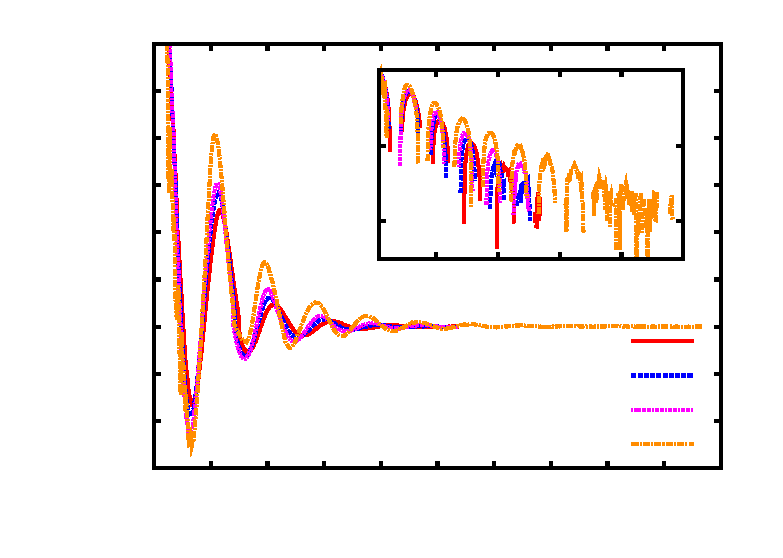
\includegraphics{g6}}%
    \gplfronttext
  \end{picture}%
\endgroup
\end{LARGE}}
	\column{0.5\textwidth}
	\begin{itemize}
		\item With coarse-graining
		\begin{itemize}
			\item Ornstein-Zernike fit
			\[ G_6(r) \propto r^{-1}\exp( -\frac{r}{\xi_6} )\]
			\item Growing correlation length
		\end{itemize}
		
		\bigskip
		\item Without coarse-graining
		\begin{itemize}
			\item Alternatively positive and negative
			\item Susceptibility $\simeq 0$
			\item No long range correlation
		\end{itemize}
	\end{itemize}
	\end{columns}
\end{frame}

\section{Crystallisation}

\begin{frame}{Crystallisation at the wall}
	\begin{columns}[T]
	\column{0.5\textwidth}
	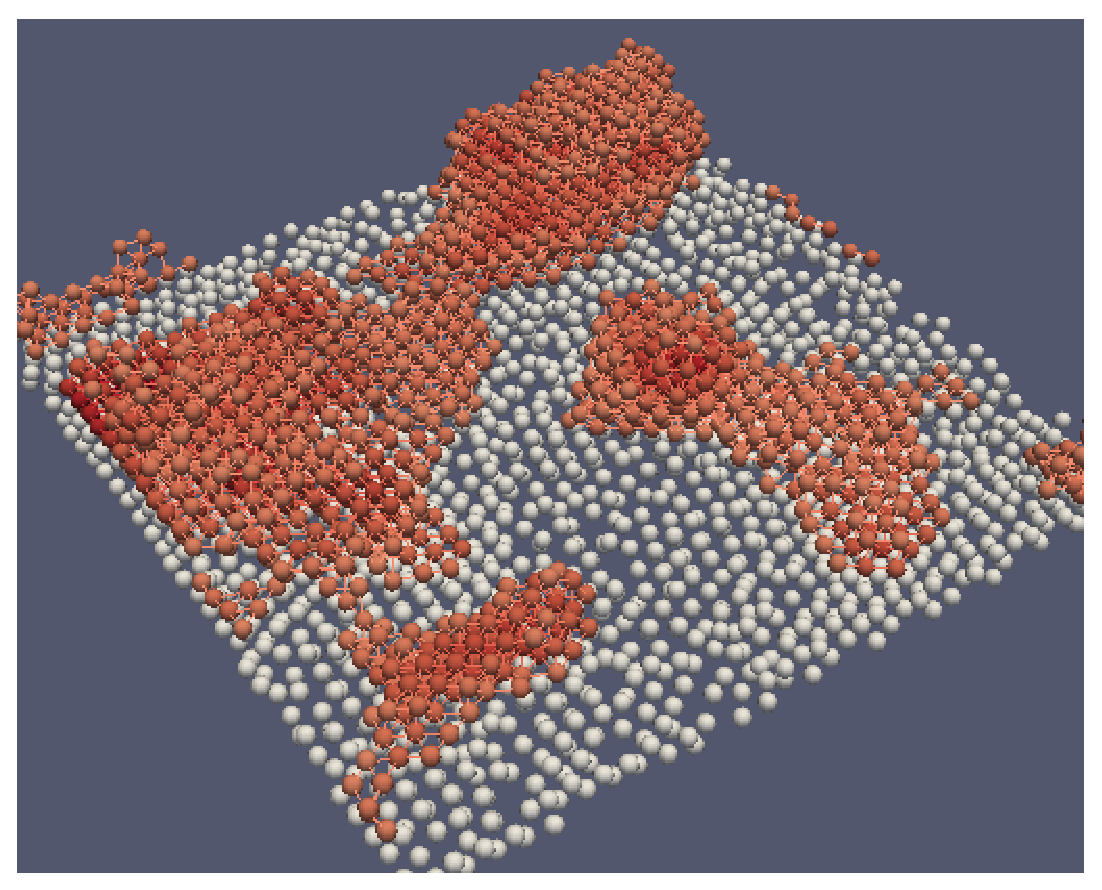
\includegraphics[width=\columnwidth]{X_mountains_Q6}\\
	\centering{Colour by degree of crystallisation ($Q_6$)}
	\column{0.5\textwidth}
	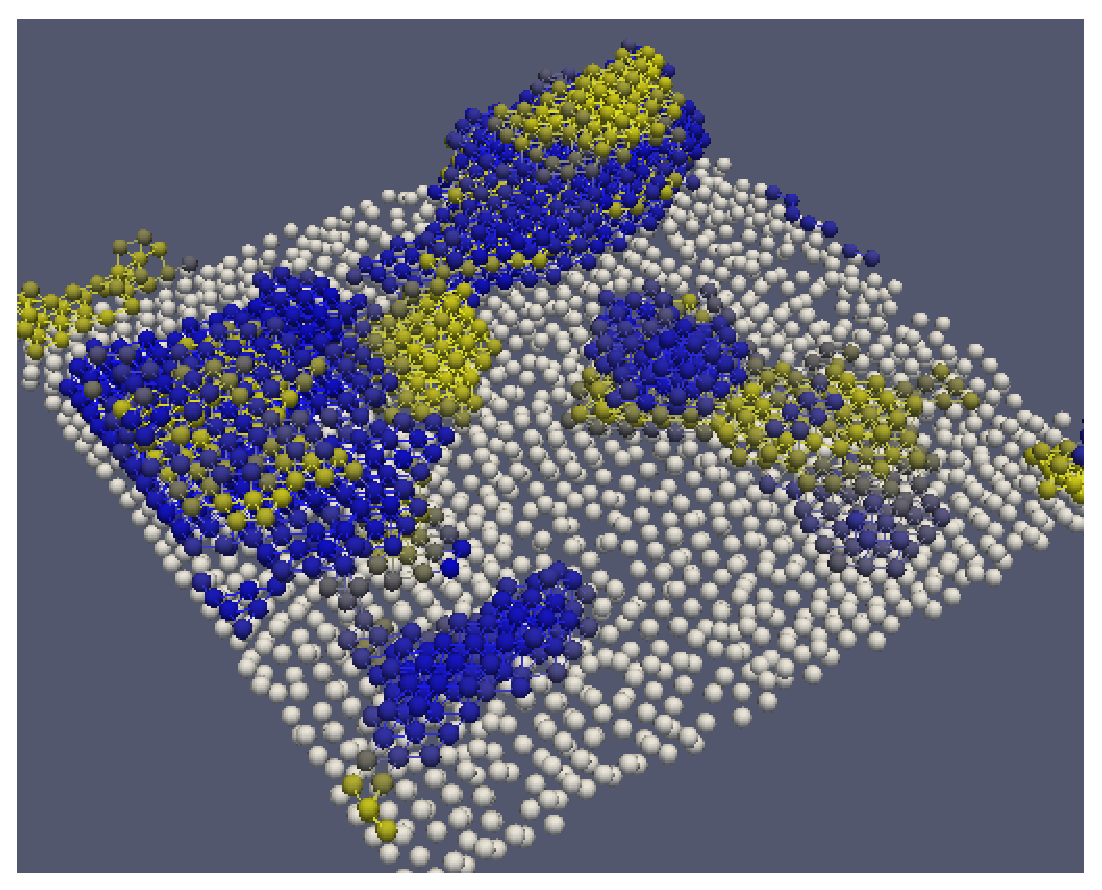
\includegraphics[width=\columnwidth]{X_mountains_W4}\\
	\tikz\shade[ball color=blue] (0,0) circle (0.5em); FCC\quad
	\tikz\shade[ball color=yellow] (0,0) circle (0.5em); HCP\quad
	($W_4$)
	\end{columns}
	\begin{itemize}
		\item Real crystals: $Q_6>0.4$
		\item Not growing homogeneously
	\end{itemize}
\end{frame}

\begin{frame}{Heterogeneous nucleation process}
	\tikz\shade[ball color=green!50!black] (0,0) circle (0.5em); $0.25<Q_6<0.4$: crystal-like order\quad
	\tikz\shade[ball color=red!50!black] (0,0) circle (0.5em); $0.4<Q_6$: crystal
	\begin{columns}
	\column{0.25\textwidth}
	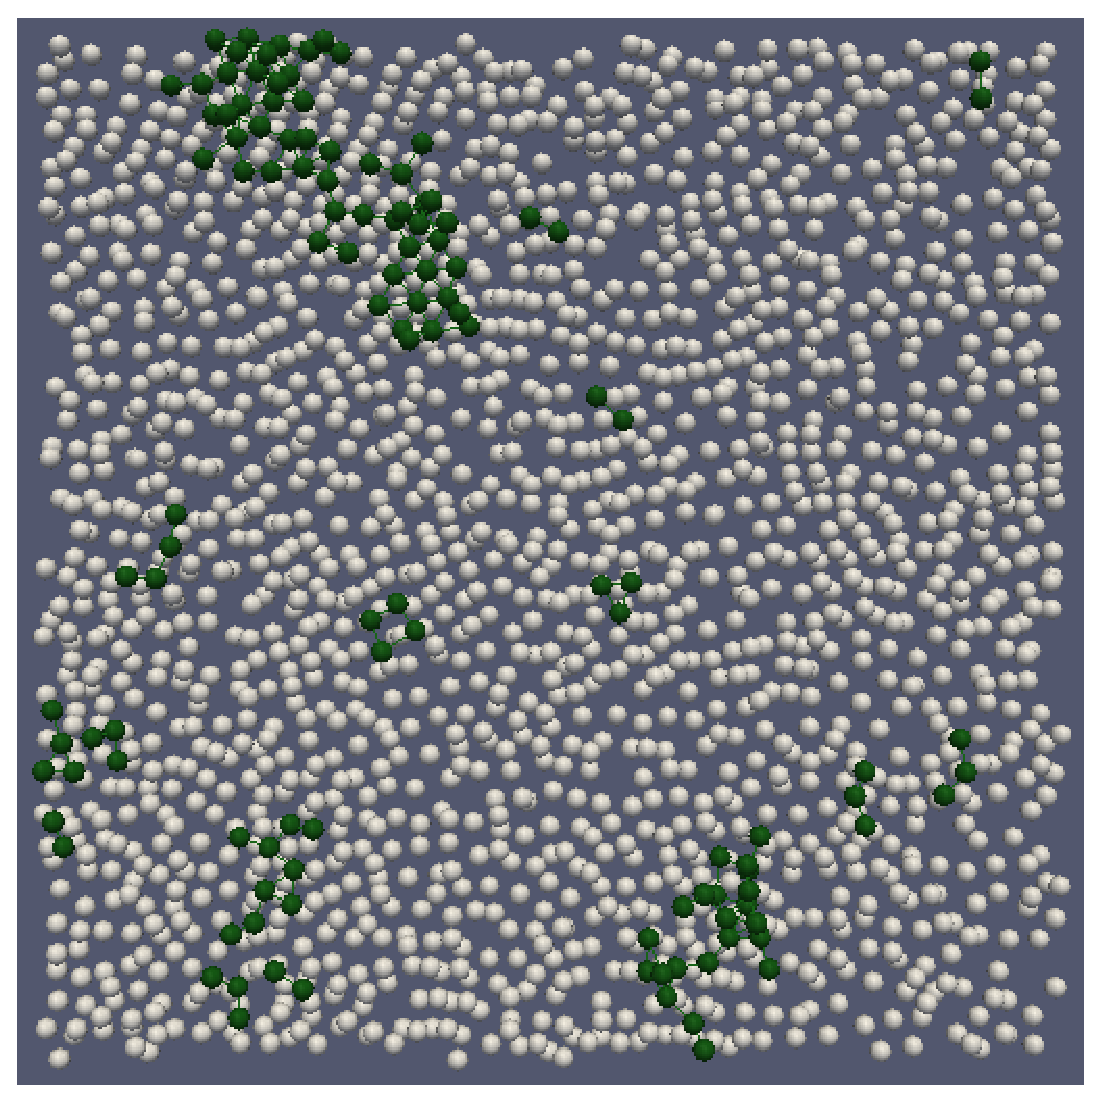
\includegraphics[width=\columnwidth]{X_t000}\\
	$t=\unit{0}{\hour}$
	
	\bigskip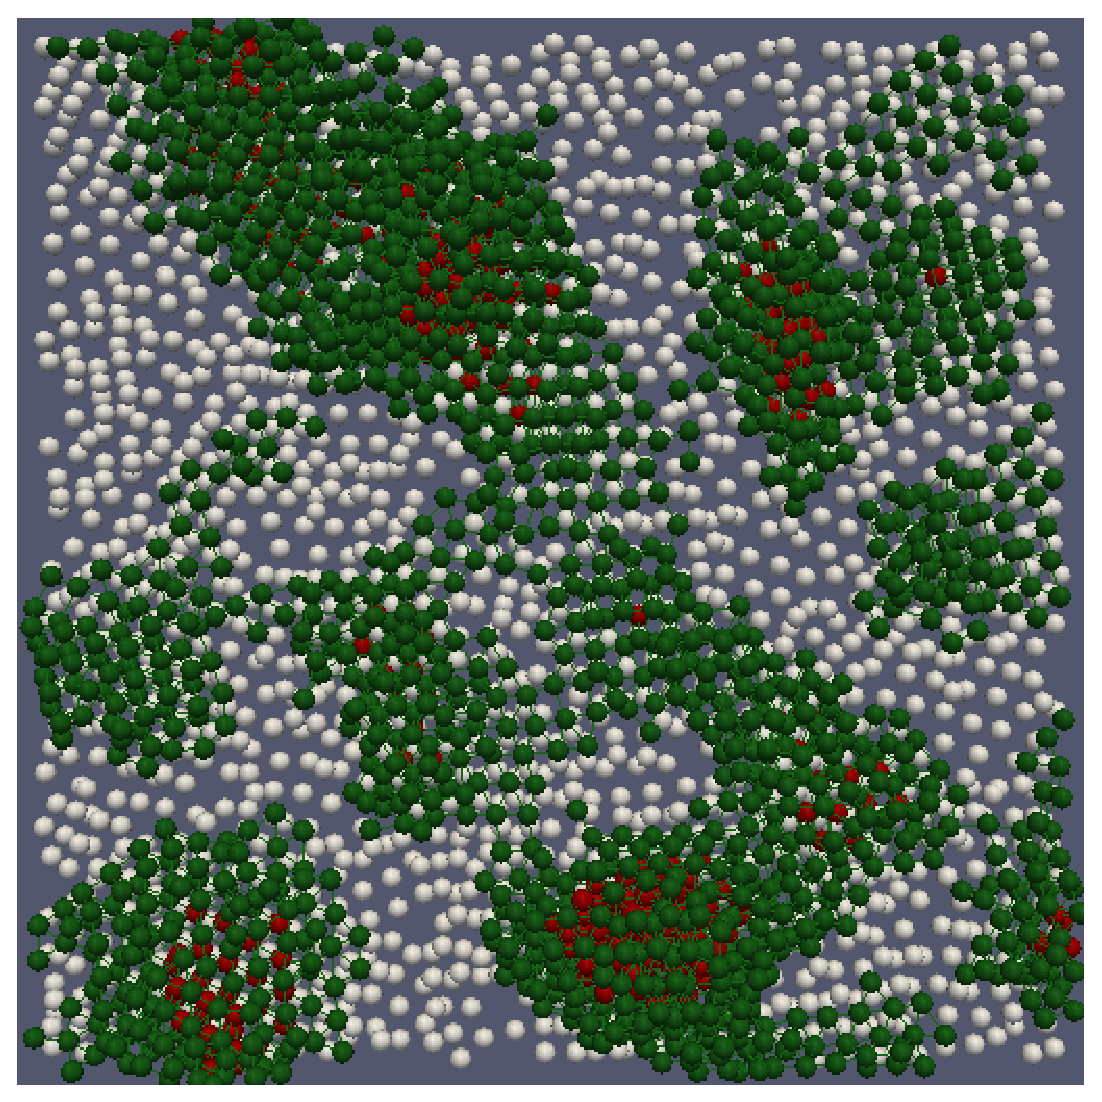
\includegraphics[width=\columnwidth]{X_t100}\\
	$t=\unit{20}{\hour}$
	%
	\column{0.25\textwidth}
	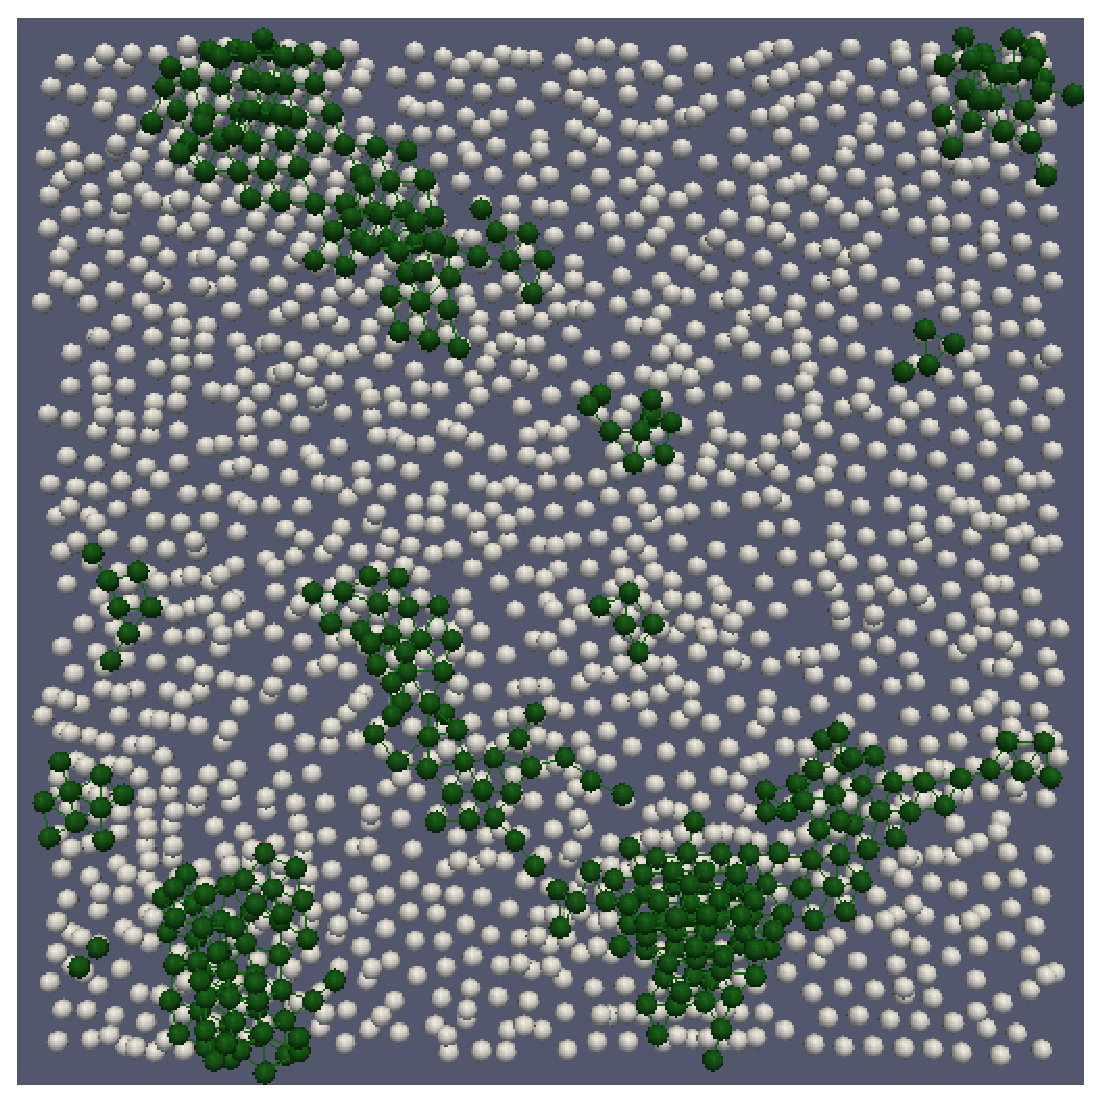
\includegraphics[width=\columnwidth]{X_t025}\\
	$t=\unit{5}{\hour}$
	
	\bigskip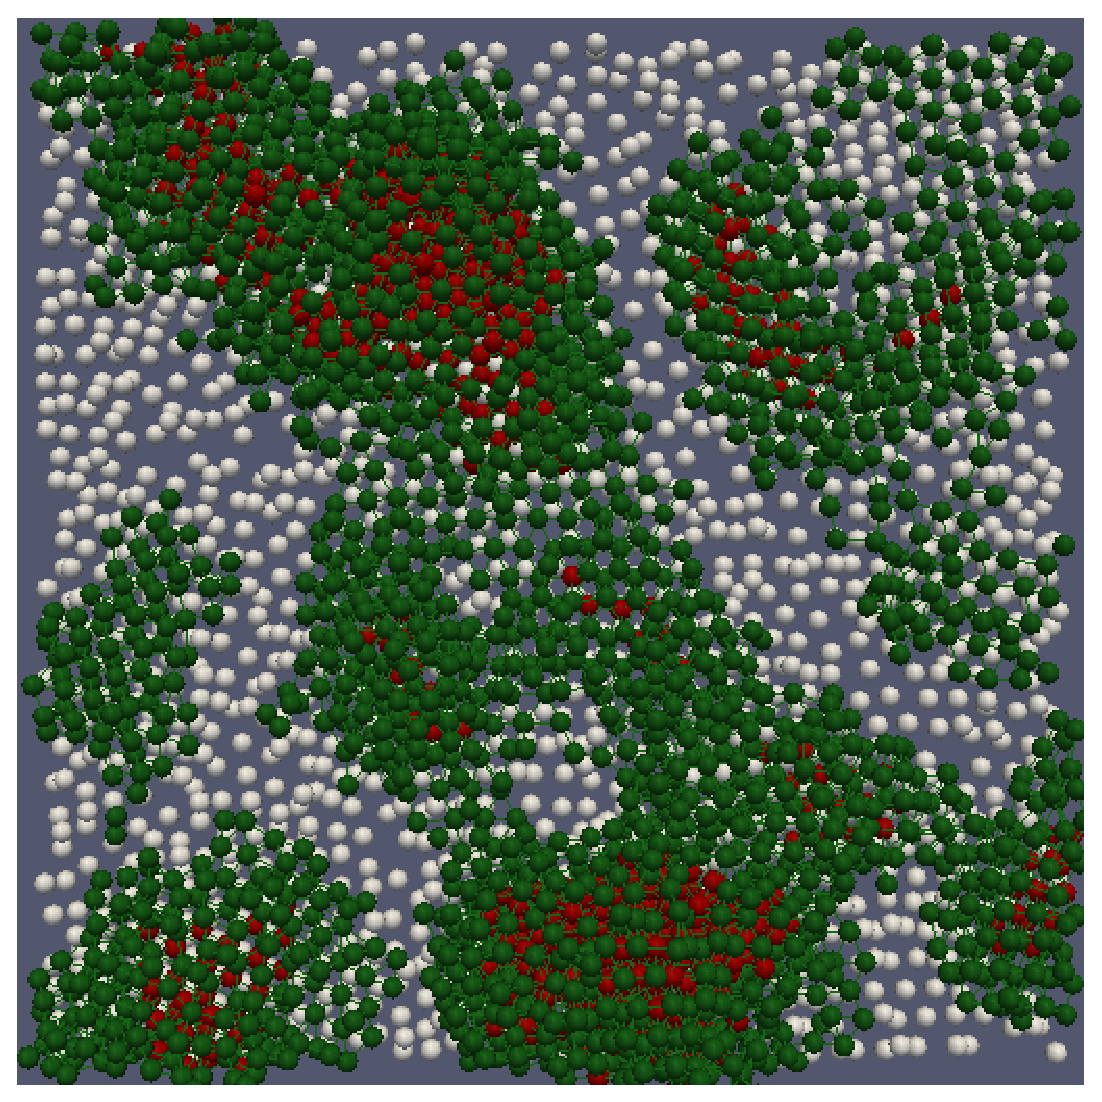
\includegraphics[width=\columnwidth]{X_t150}\\
	$t=\unit{30}{\hour}$
	%
	\column{0.25\textwidth}
	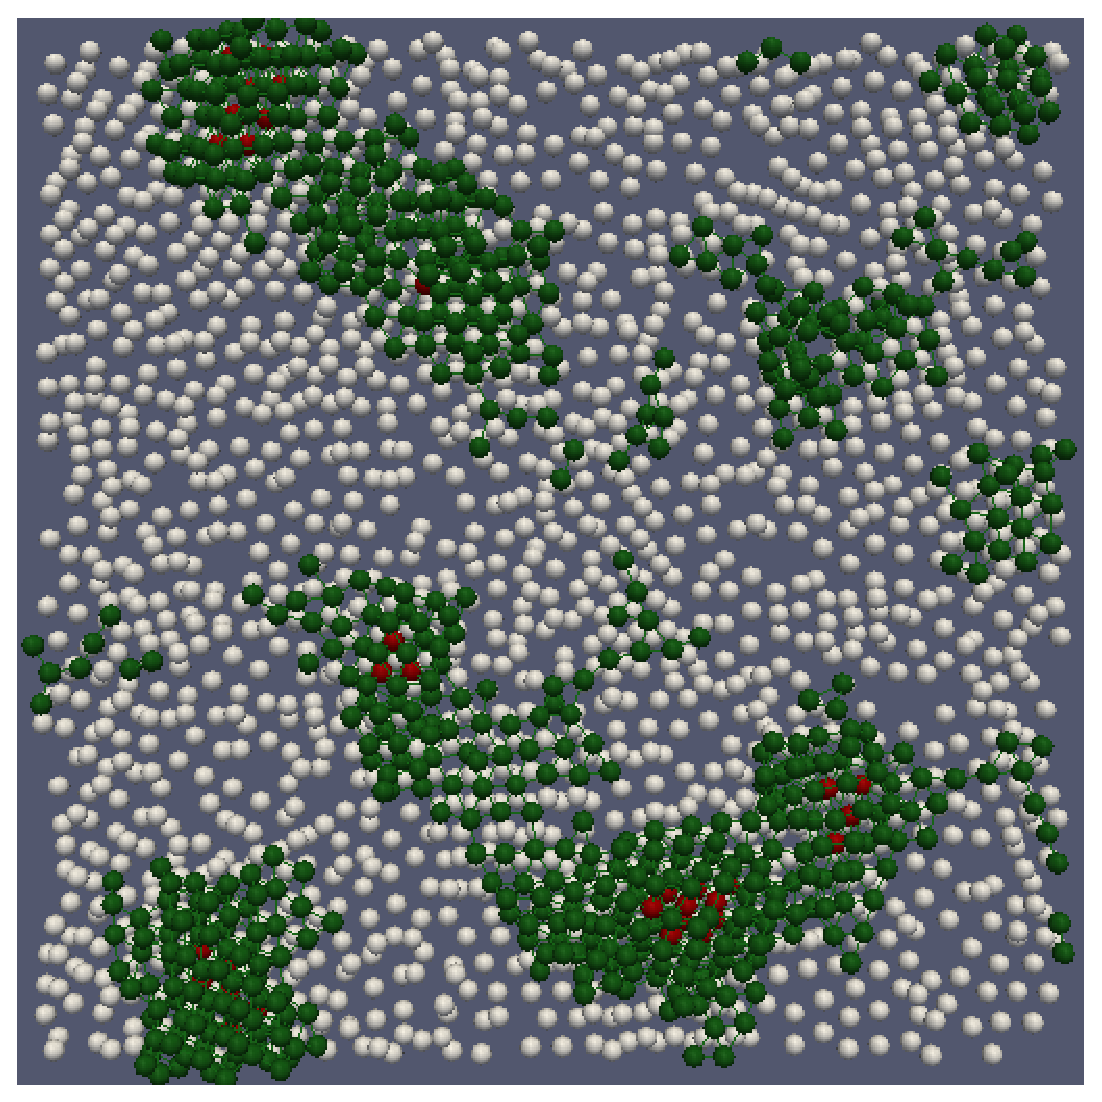
\includegraphics[width=\columnwidth]{X_t050}\\
	$t=\unit{10}{\hour}$
	
	\bigskip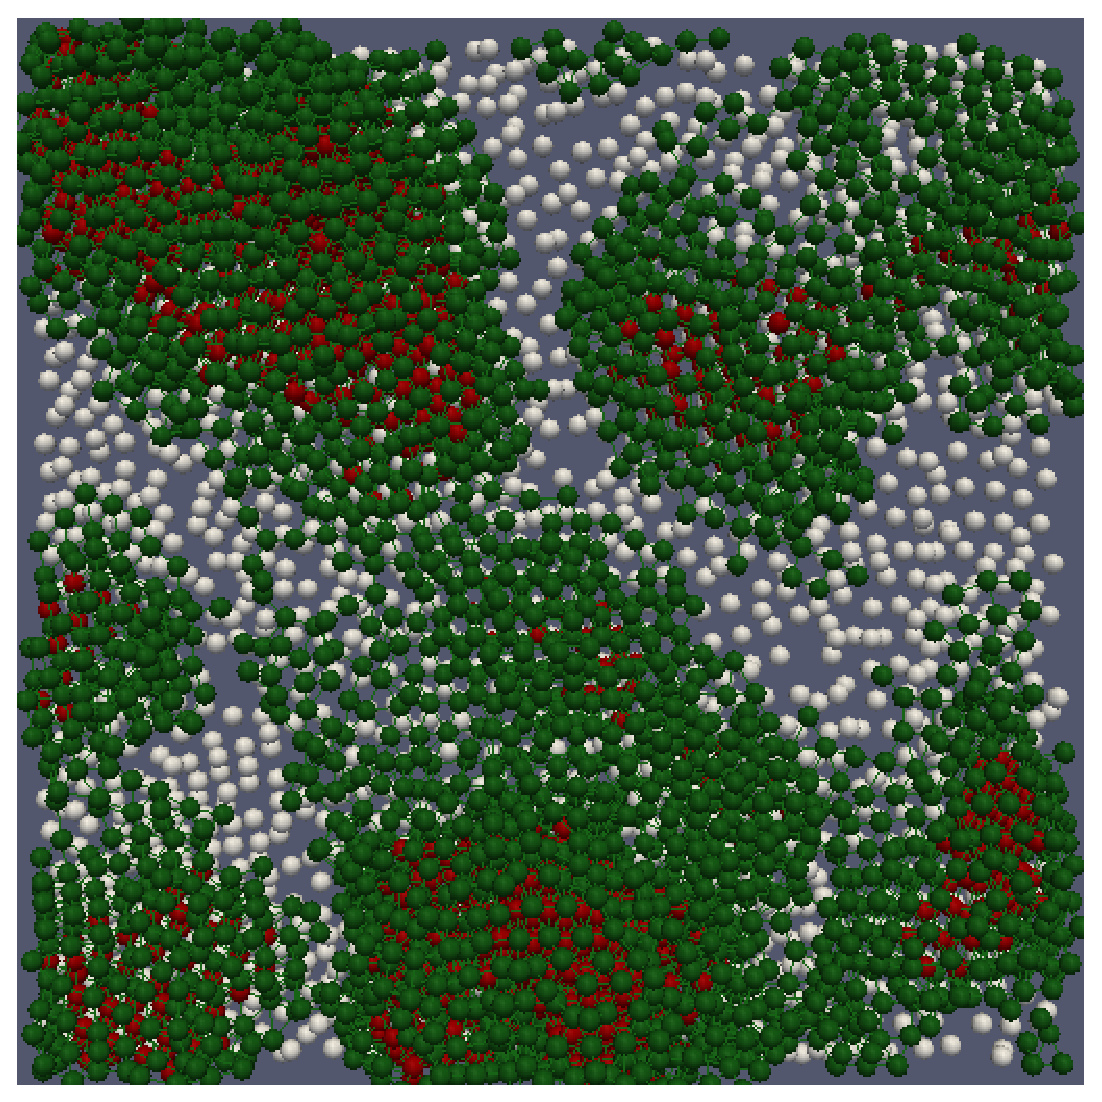
\includegraphics[width=\columnwidth]{X_t200}\\
	$t=\unit{40}{\hour}$
	%
	\column{0.25\textwidth}
	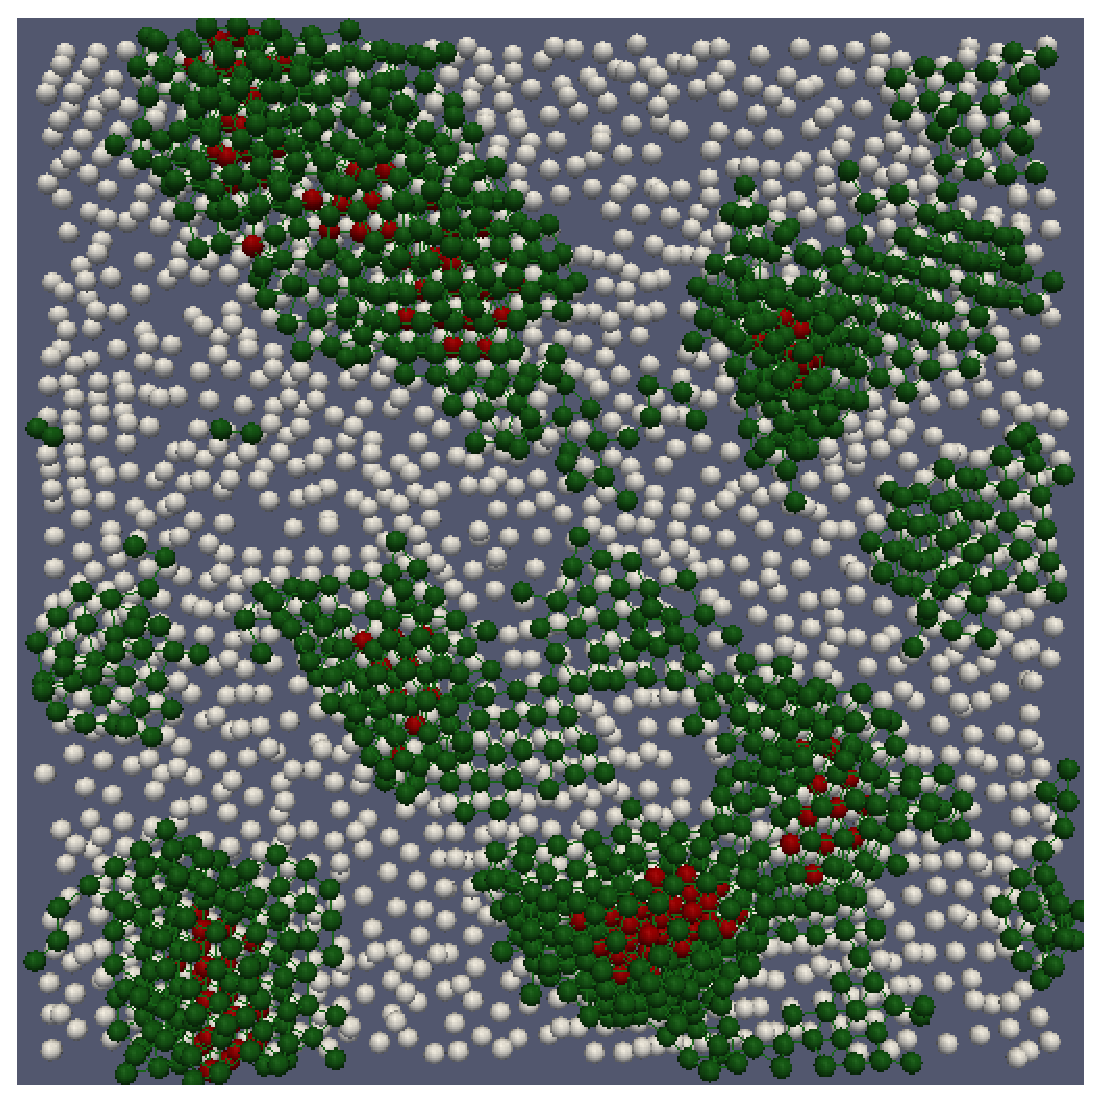
\includegraphics[width=\columnwidth]{X_t075}\\
	$t=\unit{15}{\hour}$
	
	\bigskip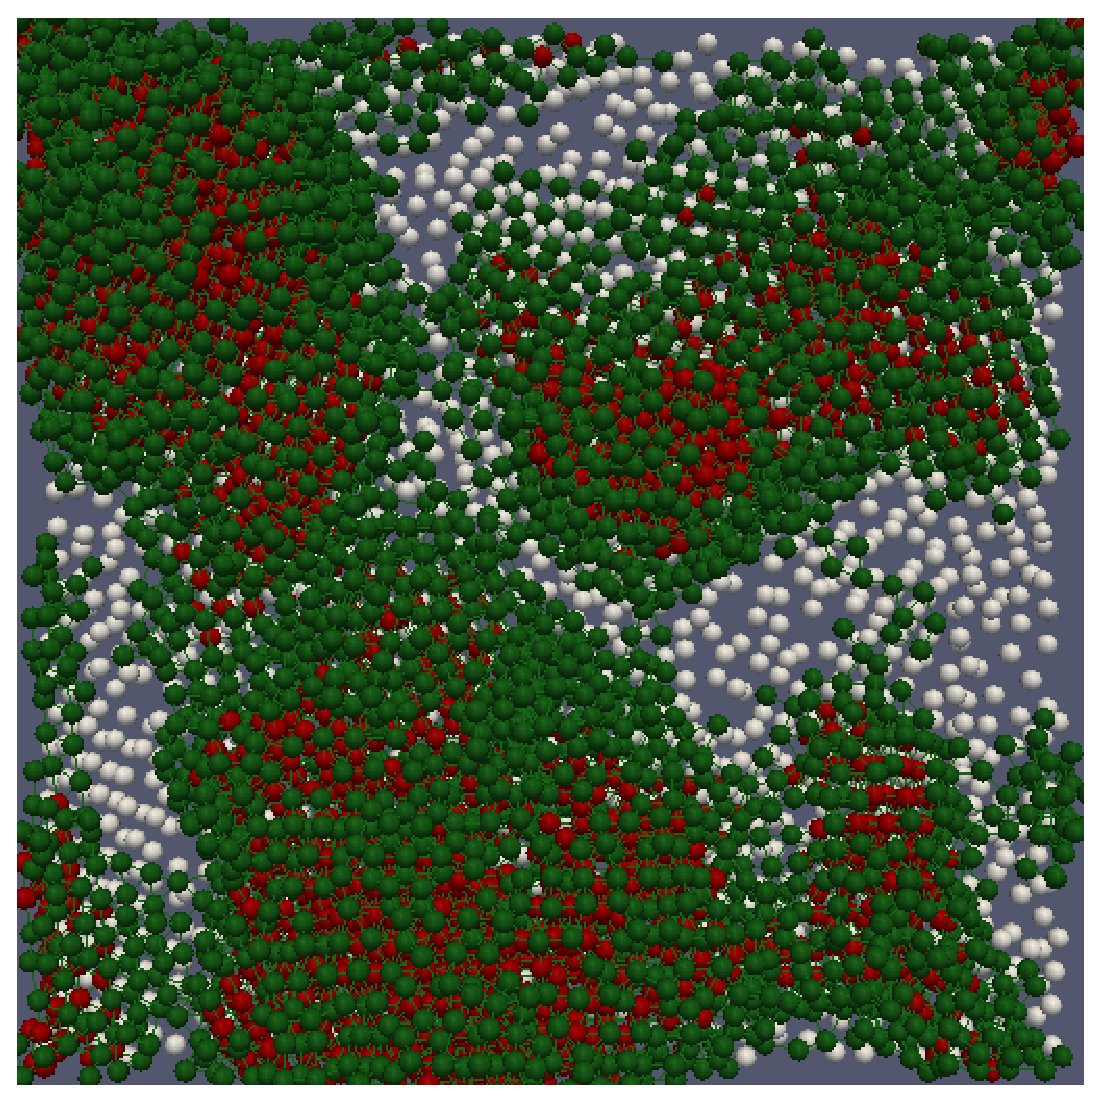
\includegraphics[width=\columnwidth]{X_t299}\\
	$t=\unit{60}{\hour}$
	\end{columns}
\end{frame}

\begin{frame}{Heterogeneous nucleation movie}
	\begin{columns}
	\column{0.6\textwidth}
	%\movie[externalviewer, inline=false, text={
		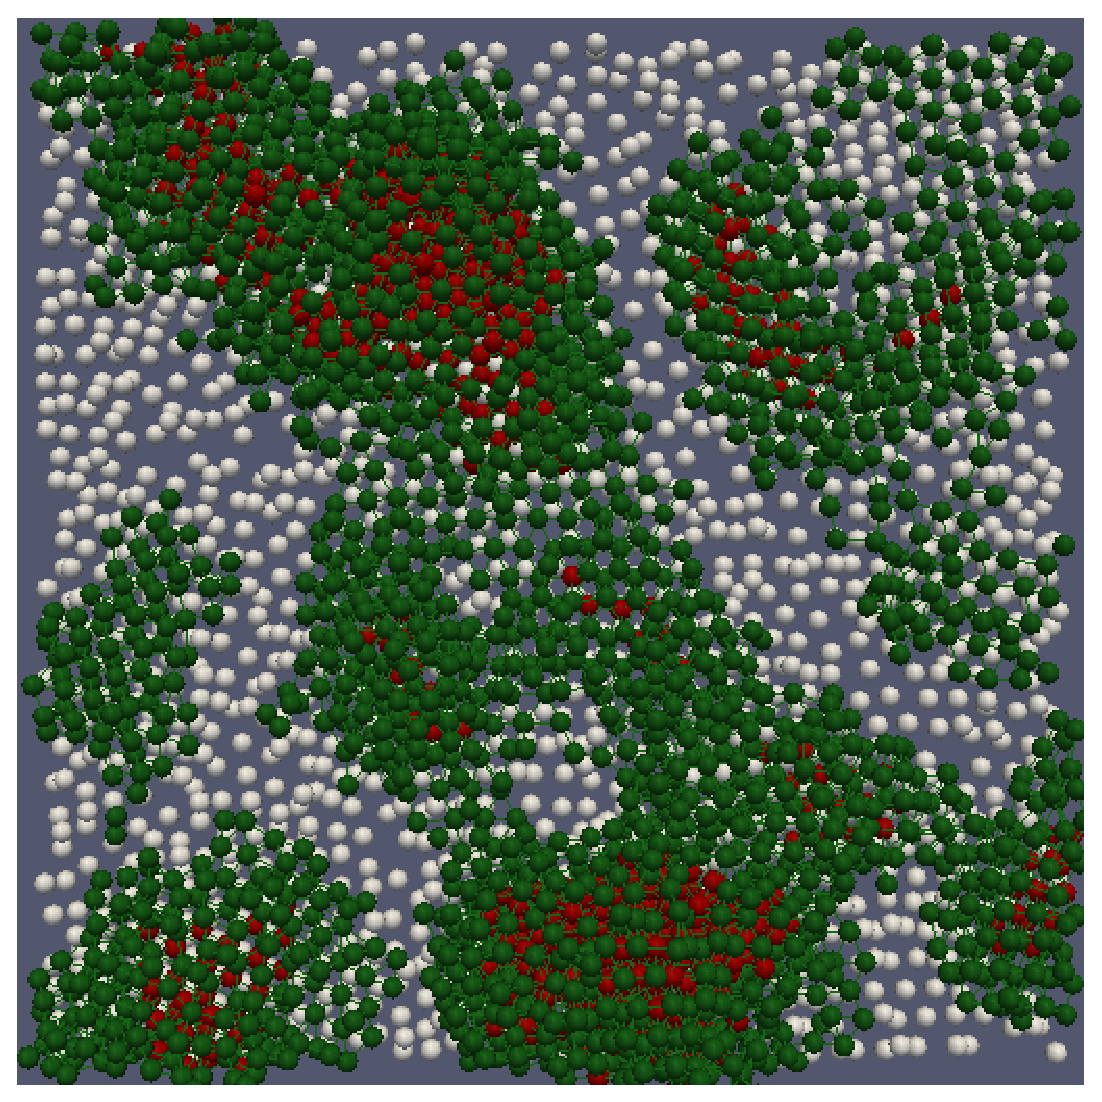
\includegraphics[width=\columnwidth]{X_t150}%}]{}{}{X.mov}
		\\
	\tikz\shade[ball color=green!50!black] (0,0) circle (0.5em); $0.25<Q_6<0.4$: crystal-like order\\
	\tikz\shade[ball color=red!50!black] (0,0) circle (0.5em); $0.4<Q_6$: crystal
	\column{0.4\textwidth}
	\begin{itemize}
		\item Bond order first
		\item Nucleation from the ordered regions
		\item $\simeq$ wetting
	\end{itemize}
	\end{columns}
\end{frame}

\begin{frame}{Density profiles}
	\centering\resizebox{0.8\textwidth}{!}{% GNUPLOT: LaTeX picture with Postscript
\begingroup
  \makeatletter
  \providecommand\color[2][]{%
    \GenericError{(gnuplot) \space\space\space\@spaces}{%
      Package color not loaded in conjunction with
      terminal option `colourtext'%
    }{See the gnuplot documentation for explanation.%
    }{Either use 'blacktext' in gnuplot or load the package
      color.sty in LaTeX.}%
    \renewcommand\color[2][]{}%
  }%
  \providecommand\includegraphics[2][]{%
    \GenericError{(gnuplot) \space\space\space\@spaces}{%
      Package graphicx or graphics not loaded%
    }{See the gnuplot documentation for explanation.%
    }{The gnuplot epslatex terminal needs graphicx.sty or graphics.sty.}%
    \renewcommand\includegraphics[2][]{}%
  }%
  \providecommand\rotatebox[2]{#2}%
  \@ifundefined{ifGPcolor}{%
    \newif\ifGPcolor
    \GPcolortrue
  }{}%
  \@ifundefined{ifGPblacktext}{%
    \newif\ifGPblacktext
    \GPblacktexttrue
  }{}%
  % define a \g@addto@macro without @ in the name:
  \let\gplgaddtomacro\g@addto@macro
  % define empty templates for all commands taking text:
  \gdef\gplbacktext{}%
  \gdef\gplfronttext{}%
  \makeatother
  \ifGPblacktext
    % no textcolor at all
    \def\colorrgb#1{}%
    \def\colorgray#1{}%
  \else
    % gray or color?
    \ifGPcolor
      \def\colorrgb#1{\color[rgb]{#1}}%
      \def\colorgray#1{\color[gray]{#1}}%
      \expandafter\def\csname LTw\endcsname{\color{white}}%
      \expandafter\def\csname LTb\endcsname{\color{black}}%
      \expandafter\def\csname LTa\endcsname{\color{black}}%
      \expandafter\def\csname LT0\endcsname{\color[rgb]{1,0,0}}%
      \expandafter\def\csname LT1\endcsname{\color[rgb]{0,1,0}}%
      \expandafter\def\csname LT2\endcsname{\color[rgb]{0,0,1}}%
      \expandafter\def\csname LT3\endcsname{\color[rgb]{1,0,1}}%
      \expandafter\def\csname LT4\endcsname{\color[rgb]{0,1,1}}%
      \expandafter\def\csname LT5\endcsname{\color[rgb]{1,1,0}}%
      \expandafter\def\csname LT6\endcsname{\color[rgb]{0,0,0}}%
      \expandafter\def\csname LT7\endcsname{\color[rgb]{1,0.3,0}}%
      \expandafter\def\csname LT8\endcsname{\color[rgb]{0.5,0.5,0.5}}%
    \else
      % gray
      \def\colorrgb#1{\color{black}}%
      \def\colorgray#1{\color[gray]{#1}}%
      \expandafter\def\csname LTw\endcsname{\color{white}}%
      \expandafter\def\csname LTb\endcsname{\color{black}}%
      \expandafter\def\csname LTa\endcsname{\color{black}}%
      \expandafter\def\csname LT0\endcsname{\color{black}}%
      \expandafter\def\csname LT1\endcsname{\color{black}}%
      \expandafter\def\csname LT2\endcsname{\color{black}}%
      \expandafter\def\csname LT3\endcsname{\color{black}}%
      \expandafter\def\csname LT4\endcsname{\color{black}}%
      \expandafter\def\csname LT5\endcsname{\color{black}}%
      \expandafter\def\csname LT6\endcsname{\color{black}}%
      \expandafter\def\csname LT7\endcsname{\color{black}}%
      \expandafter\def\csname LT8\endcsname{\color{black}}%
    \fi
  \fi
  \setlength{\unitlength}{0.0500bp}%
  \begin{picture}(7200.00,5040.00)%
    \gplgaddtomacro\gplbacktext{%
      \csname LTb\endcsname%
      \put(792,2520){\makebox(0,0)[r]{\strut{}$0.0$}}%
      \put(792,3016){\makebox(0,0)[r]{\strut{}$0.4$}}%
      \put(792,3511){\makebox(0,0)[r]{\strut{}$0.8$}}%
      \put(792,4007){\makebox(0,0)[r]{\strut{}$1.2$}}%
      \put(1625,2300){\makebox(0,0){\strut{}}}%
      \put(2501,2300){\makebox(0,0){\strut{}}}%
      \put(3377,2300){\makebox(0,0){\strut{}}}%
      \put(286,2519){\rotatebox{90}{\makebox(0,0){\strut{}Number density}}}%
      \put(4034,3449){\rotatebox{90}{\makebox(0,0){\strut{}}}}%
      \put(2369,4269){\makebox(0,0){\strut{}}}%
      \put(2369,4268){\makebox(0,0){\strut{}}}%
      \put(0,2410){\makebox(0,0)[l]{\strut{}}}%
      \put(2370,3450){\makebox(0,0){\strut{}$t=0$}}%
    }%
    \gplgaddtomacro\gplfronttext{%
      \csname LTb\endcsname%
      \put(4224,4867){\makebox(0,0)[r]{\strut{}$\rho/\langle\rho\rangle$}}%
      \csname LTb\endcsname%
      \put(4224,4647){\makebox(0,0)[r]{\strut{}$\rho_{ico}/\rho$}}%
    }%
    \gplgaddtomacro\gplbacktext{%
      \csname LTb\endcsname%
      \put(3683,2520){\makebox(0,0)[r]{\strut{}}}%
      \put(3683,3016){\makebox(0,0)[r]{\strut{}}}%
      \put(3683,3511){\makebox(0,0)[r]{\strut{}}}%
      \put(3683,4007){\makebox(0,0)[r]{\strut{}}}%
      \put(4572,2300){\makebox(0,0){\strut{}}}%
      \put(5517,2300){\makebox(0,0){\strut{}}}%
      \put(6463,2300){\makebox(0,0){\strut{}}}%
      \put(7155,3449){\rotatebox{90}{\makebox(0,0){\strut{}}}}%
      \put(5375,4269){\makebox(0,0){\strut{}}}%
      \put(5375,4268){\makebox(0,0){\strut{}}}%
      \put(3551,2410){\makebox(0,0)[l]{\strut{}}}%
      \put(5376,3450){\makebox(0,0){\strut{}$t=\unit{10}{\hour}$}}%
    }%
    \gplgaddtomacro\gplfronttext{%
      \csname LTb\endcsname%
      \put(6191,4867){\makebox(0,0)[r]{\strut{}$\rho_{mrco}/\rho$}}%
      \csname LTb\endcsname%
      \put(6191,4647){\makebox(0,0)[r]{\strut{}$\rho_X/\rho$}}%
    }%
    \gplgaddtomacro\gplbacktext{%
      \csname LTb\endcsname%
      \put(792,704){\makebox(0,0)[r]{\strut{}$0.0$}}%
      \put(792,1188){\makebox(0,0)[r]{\strut{}$0.4$}}%
      \put(792,1672){\makebox(0,0)[r]{\strut{}$0.8$}}%
      \put(792,2156){\makebox(0,0)[r]{\strut{}$1.2$}}%
      \put(1625,484){\makebox(0,0){\strut{}$10$}}%
      \put(2501,484){\makebox(0,0){\strut{}$20$}}%
      \put(3377,484){\makebox(0,0){\strut{}$30$}}%
      \put(4034,1611){\rotatebox{90}{\makebox(0,0){\strut{}}}}%
      \put(2369,154){\makebox(0,0){\strut{}$z/\sigma$}}%
      \put(2369,2409){\makebox(0,0){\strut{}}}%
      \put(2369,2408){\makebox(0,0){\strut{}}}%
      \put(0,110){\makebox(0,0)[l]{\strut{}}}%
      \put(2370,1612){\makebox(0,0){\strut{}$t=\unit{30}{\hour}$}}%
    }%
    \gplgaddtomacro\gplfronttext{%
    }%
    \gplgaddtomacro\gplbacktext{%
      \csname LTb\endcsname%
      \put(3683,704){\makebox(0,0)[r]{\strut{}}}%
      \put(3683,1188){\makebox(0,0)[r]{\strut{}}}%
      \put(3683,1672){\makebox(0,0)[r]{\strut{}}}%
      \put(3683,2156){\makebox(0,0)[r]{\strut{}}}%
      \put(4572,484){\makebox(0,0){\strut{}$10$}}%
      \put(5517,484){\makebox(0,0){\strut{}$20$}}%
      \put(6463,484){\makebox(0,0){\strut{}$30$}}%
      \put(7155,1611){\rotatebox{90}{\makebox(0,0){\strut{}}}}%
      \put(5375,154){\makebox(0,0){\strut{}$z/\sigma$}}%
      \put(5375,2409){\makebox(0,0){\strut{}}}%
      \put(5375,2408){\makebox(0,0){\strut{}}}%
      \put(3551,110){\makebox(0,0)[l]{\strut{}}}%
      \put(5376,1612){\makebox(0,0){\strut{}$t=\unit{60}{\hour}$}}%
    }%
    \gplgaddtomacro\gplfronttext{%
    }%
    \gplbacktext
    \put(0,0){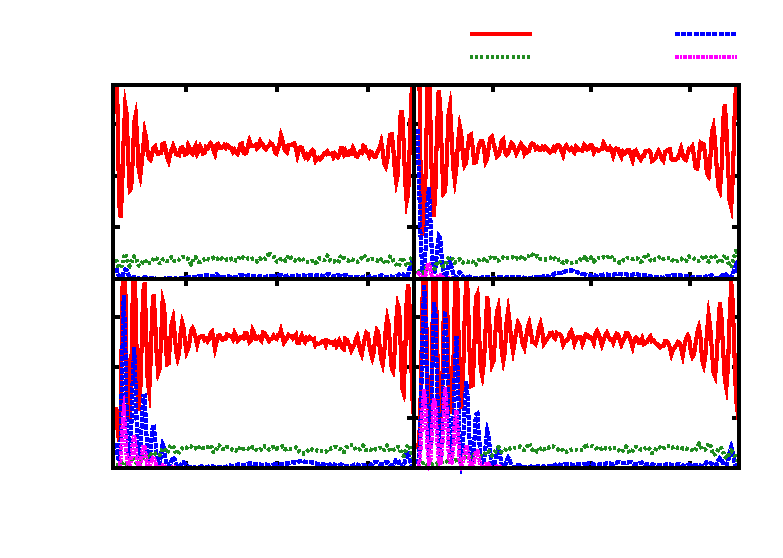
\includegraphics{X_profile}}%
    \gplfronttext
  \end{picture}%
\endgroup
}
	\begin{itemize}
		\item Layering at the wall
		\item Icosahedra's centres are also layered
	\end{itemize}
\end{frame}

\begin{frame}{Normalised density profiles}
	\begin{columns}
	\column{0.5\textwidth}
	\resizebox{\columnwidth}{!}{% GNUPLOT: LaTeX picture with Postscript
\begingroup
  \makeatletter
  \providecommand\color[2][]{%
    \GenericError{(gnuplot) \space\space\space\@spaces}{%
      Package color not loaded in conjunction with
      terminal option `colourtext'%
    }{See the gnuplot documentation for explanation.%
    }{Either use 'blacktext' in gnuplot or load the package
      color.sty in LaTeX.}%
    \renewcommand\color[2][]{}%
  }%
  \providecommand\includegraphics[2][]{%
    \GenericError{(gnuplot) \space\space\space\@spaces}{%
      Package graphicx or graphics not loaded%
    }{See the gnuplot documentation for explanation.%
    }{The gnuplot epslatex terminal needs graphicx.sty or graphics.sty.}%
    \renewcommand\includegraphics[2][]{}%
  }%
  \providecommand\rotatebox[2]{#2}%
  \@ifundefined{ifGPcolor}{%
    \newif\ifGPcolor
    \GPcolortrue
  }{}%
  \@ifundefined{ifGPblacktext}{%
    \newif\ifGPblacktext
    \GPblacktexttrue
  }{}%
  % define a \g@addto@macro without @ in the name:
  \let\gplgaddtomacro\g@addto@macro
  % define empty templates for all commands taking text:
  \gdef\gplbacktext{}%
  \gdef\gplfronttext{}%
  \makeatother
  \ifGPblacktext
    % no textcolor at all
    \def\colorrgb#1{}%
    \def\colorgray#1{}%
  \else
    % gray or color?
    \ifGPcolor
      \def\colorrgb#1{\color[rgb]{#1}}%
      \def\colorgray#1{\color[gray]{#1}}%
      \expandafter\def\csname LTw\endcsname{\color{white}}%
      \expandafter\def\csname LTb\endcsname{\color{black}}%
      \expandafter\def\csname LTa\endcsname{\color{black}}%
      \expandafter\def\csname LT0\endcsname{\color[rgb]{1,0,0}}%
      \expandafter\def\csname LT1\endcsname{\color[rgb]{0,1,0}}%
      \expandafter\def\csname LT2\endcsname{\color[rgb]{0,0,1}}%
      \expandafter\def\csname LT3\endcsname{\color[rgb]{1,0,1}}%
      \expandafter\def\csname LT4\endcsname{\color[rgb]{0,1,1}}%
      \expandafter\def\csname LT5\endcsname{\color[rgb]{1,1,0}}%
      \expandafter\def\csname LT6\endcsname{\color[rgb]{0,0,0}}%
      \expandafter\def\csname LT7\endcsname{\color[rgb]{1,0.3,0}}%
      \expandafter\def\csname LT8\endcsname{\color[rgb]{0.5,0.5,0.5}}%
    \else
      % gray
      \def\colorrgb#1{\color{black}}%
      \def\colorgray#1{\color[gray]{#1}}%
      \expandafter\def\csname LTw\endcsname{\color{white}}%
      \expandafter\def\csname LTb\endcsname{\color{black}}%
      \expandafter\def\csname LTa\endcsname{\color{black}}%
      \expandafter\def\csname LT0\endcsname{\color{black}}%
      \expandafter\def\csname LT1\endcsname{\color{black}}%
      \expandafter\def\csname LT2\endcsname{\color{black}}%
      \expandafter\def\csname LT3\endcsname{\color{black}}%
      \expandafter\def\csname LT4\endcsname{\color{black}}%
      \expandafter\def\csname LT5\endcsname{\color{black}}%
      \expandafter\def\csname LT6\endcsname{\color{black}}%
      \expandafter\def\csname LT7\endcsname{\color{black}}%
      \expandafter\def\csname LT8\endcsname{\color{black}}%
    \fi
  \fi
  \setlength{\unitlength}{0.0500bp}%
  \begin{picture}(7200.00,5040.00)%
    \gplgaddtomacro\gplbacktext{%
      \csname LTb\endcsname%
      \put(924,704){\makebox(0,0)[r]{\strut{}$0$}}%
      \put(924,1259){\makebox(0,0)[r]{\strut{}$0.2$}}%
      \put(924,1813){\makebox(0,0)[r]{\strut{}$0.4$}}%
      \put(924,2368){\makebox(0,0)[r]{\strut{}$0.6$}}%
      \put(924,2922){\makebox(0,0)[r]{\strut{}$0.8$}}%
      \put(924,3477){\makebox(0,0)[r]{\strut{}$1$}}%
      \put(924,4031){\makebox(0,0)[r]{\strut{}$1.2$}}%
      \put(1056,484){\makebox(0,0){\strut{}$2$}}%
      \put(1934,484){\makebox(0,0){\strut{}$4$}}%
      \put(2811,484){\makebox(0,0){\strut{}$6$}}%
      \put(3689,484){\makebox(0,0){\strut{}$8$}}%
      \put(4566,484){\makebox(0,0){\strut{}$10$}}%
      \put(5444,484){\makebox(0,0){\strut{}$12$}}%
      \put(6321,484){\makebox(0,0){\strut{}$14$}}%
      \put(286,2367){\rotatebox{90}{\makebox(0,0){\strut{}Number density}}}%
      \put(6979,2367){\rotatebox{90}{\makebox(0,0){\strut{}}}}%
      \put(3908,154){\makebox(0,0){\strut{}$z/\sigma$}}%
      \put(3908,3921){\makebox(0,0){\strut{}}}%
      \put(3908,3920){\makebox(0,0){\strut{}}}%
      \put(132,110){\makebox(0,0)[l]{\strut{}}}%
      \put(3908,3366){\makebox(0,0){\strut{}$t=\unit{40}{\hour}$}}%
    }%
    \gplgaddtomacro\gplfronttext{%
      \csname LTb\endcsname%
      \put(5773,2697){\makebox(0,0)[r]{\strut{}$\rho_{mrco}/\rho$}}%
      \csname LTb\endcsname%
      \put(5773,2367){\makebox(0,0)[r]{\strut{}$\rho_{ico}/\rho$}}%
      \csname LTb\endcsname%
      \put(5773,2037){\makebox(0,0)[r]{\strut{}$\rho_{ico}/(\rho-\rho_{mrco})$}}%
    }%
    \gplgaddtomacro\gplbacktext{%
      \csname LTb\endcsname%
      \put(924,4294){\makebox(0,0)[r]{\strut{}$0.1$}}%
      \put(924,4557){\makebox(0,0)[r]{\strut{}$0.2$}}%
      \put(924,4819){\makebox(0,0)[r]{\strut{}$0.3$}}%
      \put(1056,3812){\makebox(0,0){\strut{}}}%
      \put(1934,3812){\makebox(0,0){\strut{}}}%
      \put(2811,3812){\makebox(0,0){\strut{}}}%
      \put(3689,3812){\makebox(0,0){\strut{}}}%
      \put(4566,3812){\makebox(0,0){\strut{}}}%
      \put(5444,3812){\makebox(0,0){\strut{}}}%
      \put(6321,3812){\makebox(0,0){\strut{}}}%
      \put(6979,4425){\rotatebox{90}{\makebox(0,0){\strut{}}}}%
      \put(3908,4709){\makebox(0,0){\strut{}}}%
      \put(3908,4708){\makebox(0,0){\strut{}}}%
      \put(132,3922){\makebox(0,0)[l]{\strut{}}}%
      \put(3908,4662){\makebox(0,0){\strut{}$t=0$}}%
    }%
    \gplgaddtomacro\gplfronttext{%
    }%
    \gplbacktext
    \put(0,0){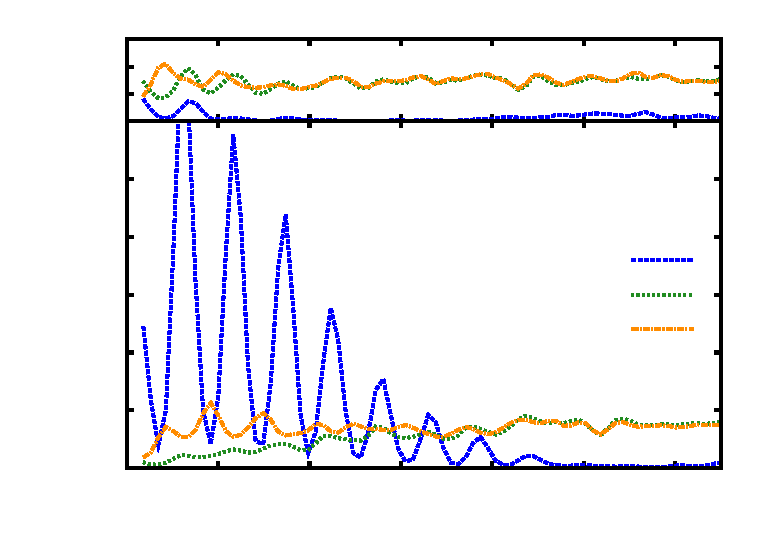
\includegraphics{X_profile_normed}}%
    \gplfronttext
  \end{picture}%
\endgroup
}
	\column{0.5\textwidth}
	\begin{itemize}
		\item Normalise by the volume available to the icosahedron
		\item Excluded from crystal-like order
	\end{itemize}
	\end{columns}
	\begin{itemize}
		\item Icosahedral order penetrate deep in the valley between the nucleus
		\item Icosahedra fit better between the layers
	\end{itemize}
\end{frame}